% !TEX root = ../thesis.tex

\chapter{Neural network triggers}
\label{chap:neural-network-triggers}

\section{Motivation}
\label{sec:motivation}

The station-level triggers in the previous chapter have been shown to perform well for the science case of the Pierre Auger Observatory. However, it has also been
concluded that potential significant discoveries might be made at energies currently outside of the sensitive region of the detector. The data of many low energy 
events is not read out by intention in order to keep DAQ readout at feasible levels.

Attempts at improving the overal efficiency of the SD triggers can be made. This is only possible to a certain level. At lowest energies, the particle cascade is 
not big enough to result in coincident triggers in at least 3 WCD stations. As per \autoref{sssec:bayesian-folding}, the lateral trigger probability a given 
classification algorithm can maximally achieve is given by the LPP (c.f. \autoref{fig:fitfunction-comparison}). The T3 detection probability of such an ideal 
trigger, and consequently the maximal efficiency for an array with $\SI{1.5}{\kilo\meter}$ spacing is compared to the efficiency of classical triggers in 
\autoref{fig:classical-trigger-performance}.

Of course, efficiency can be improved simply by adjusting trigger thresholds of the algorithms in \autoref{sec:trigger-implementation}. However, the more lenient
these thresholds are, the more background events will be detected. This quickly results in trigger rates that are unmanagable for the infrastructure at the Pierre 
Auger observatory. The probability with which time traces correctly raise a T2 is shown alongside the resulting random-trace trigger rate for different thresholds
of classical algorithms in \autoref{fig:classical-trigger-performance}.

Ideally, neural network architectures developed in this chapter should undercut the random-trace trigger rate of classical triggers, while retaining an overall 
higher accuracy. That is, they lay below and right of the operating point in \autoref{fig:classical-trigger-performance}. For any algorithm that achieves this, the 
corresponding LTP will be greater than that of classical triggers, resulting in higher event detection efficiency, while not exceeding the bandwidth limitations 
of the underlying hardware. 

\begin{figure}
	\centering
	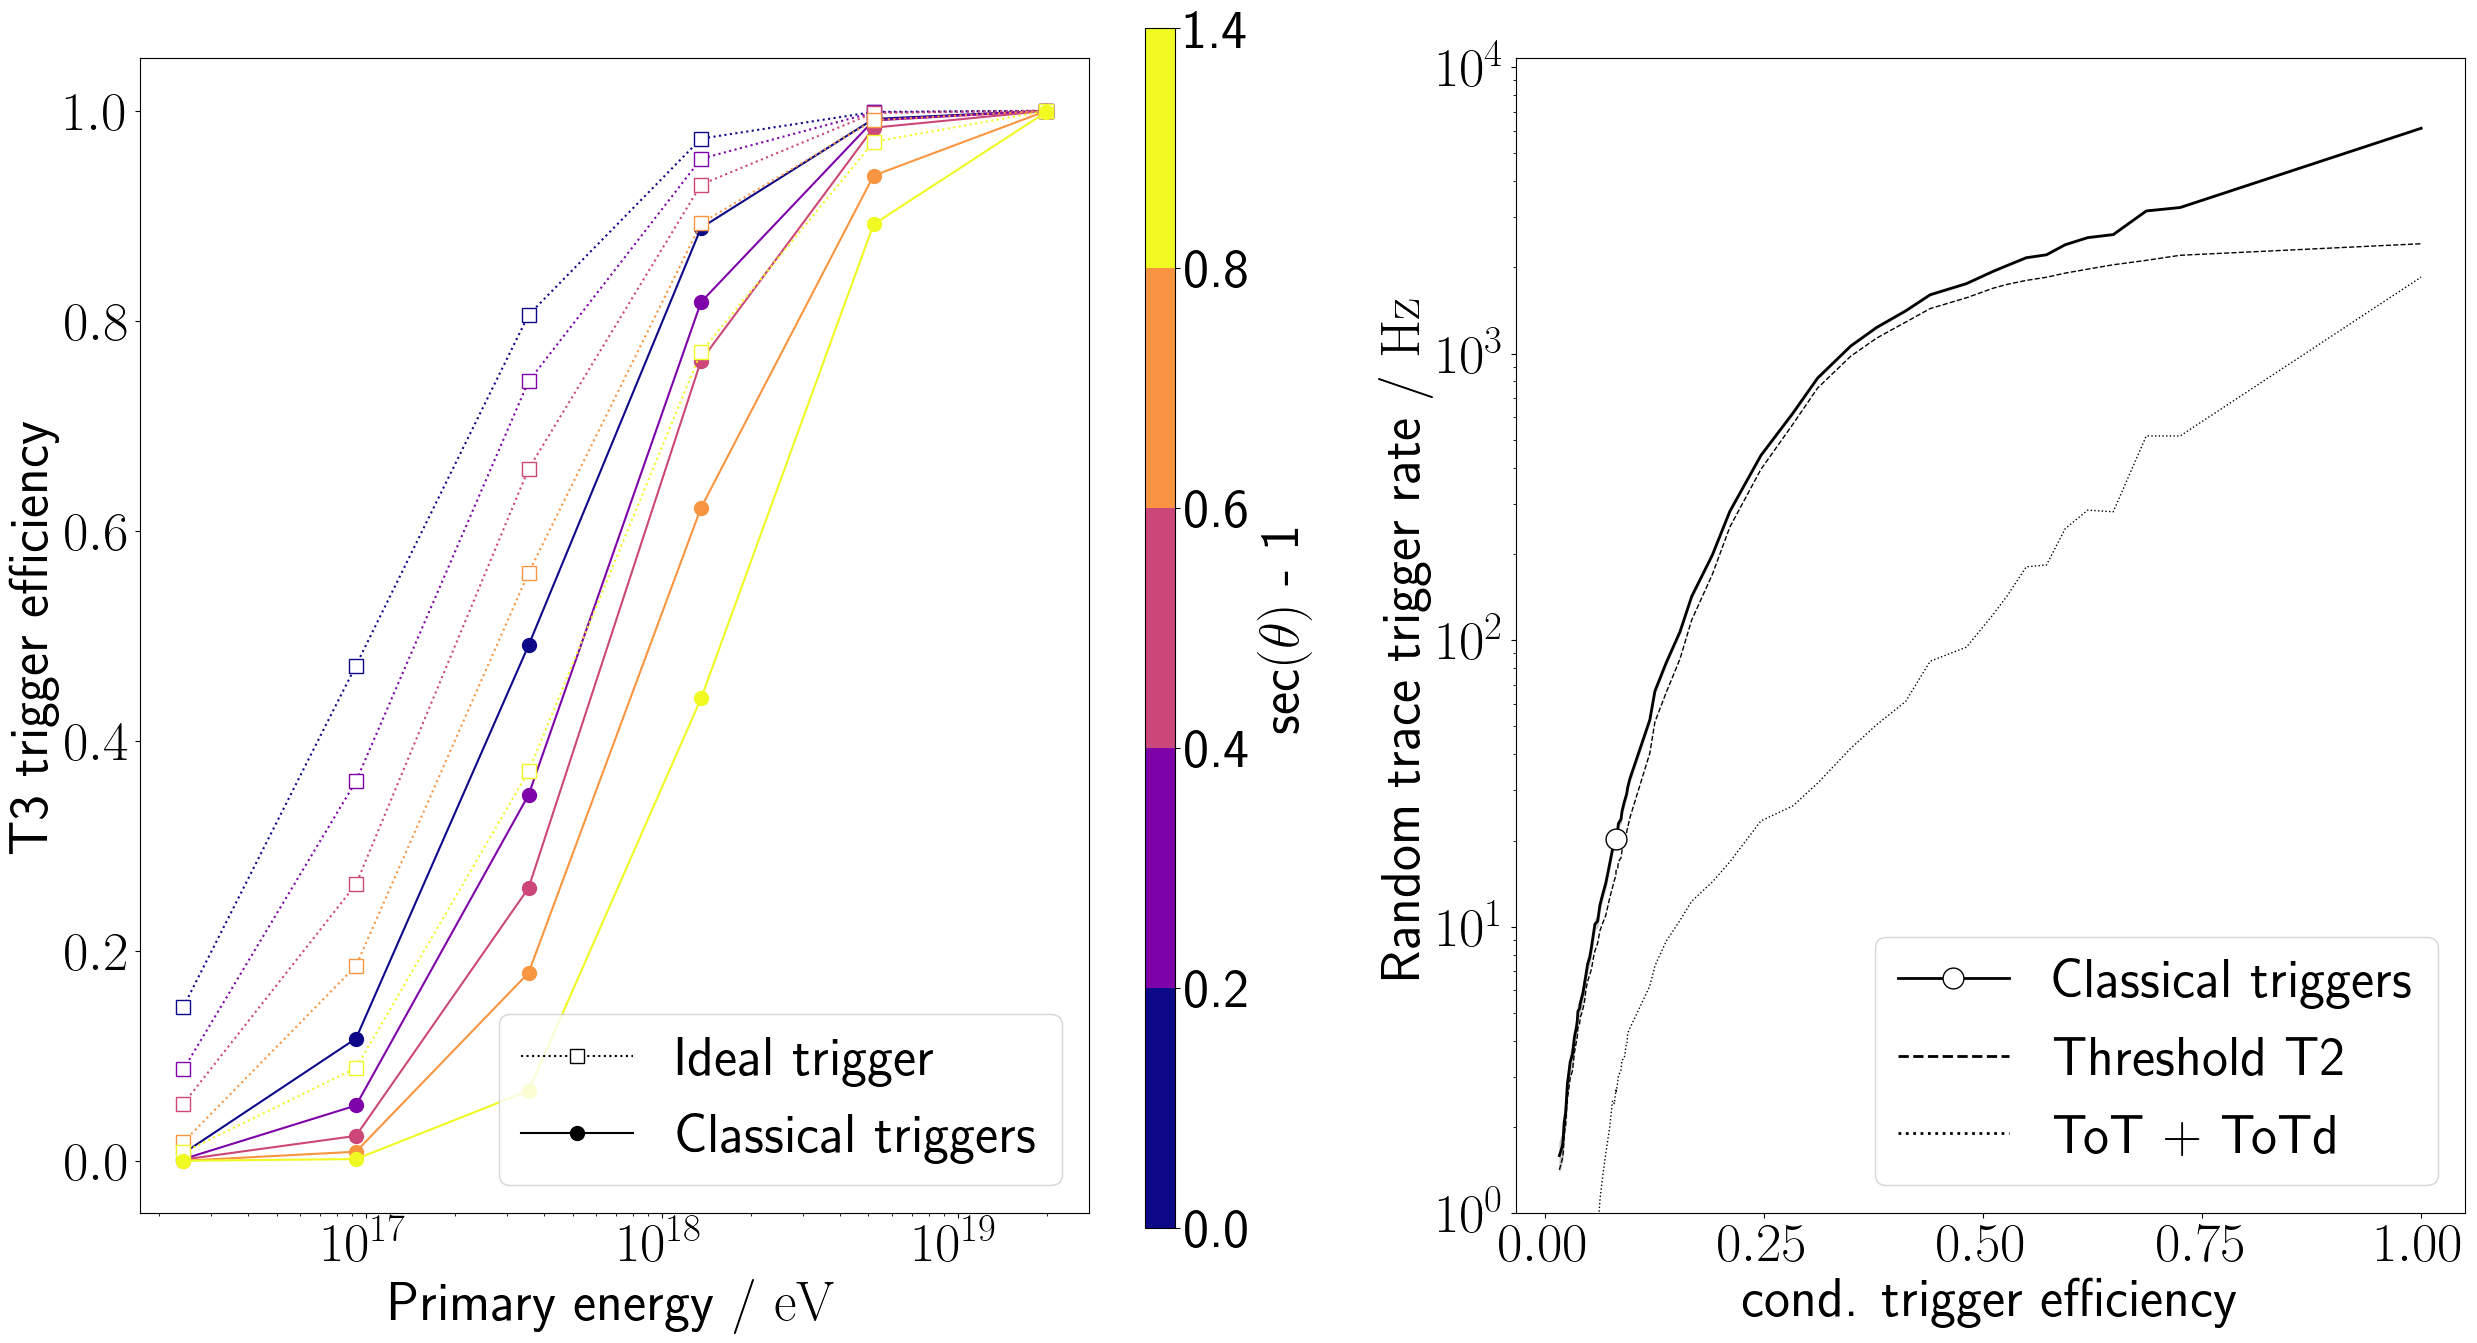
\includegraphics[width=1\textwidth]{./plots/classical_triggers.png}
	\caption{(\textit{Left}) Comparison of an ideal trigger sensitive to any shower signal from primary energies $E\geq\SI{10}{\peta\electronvolt}$ to classical 
    triggers. (\textit{Right}) The noise level over calculated efficiency for classical triggers. The tail ends of the potential curve are calculated by adjusting 
	the trigger thresholds from $0.05$ to $2.5$ times of the nominal values. The black circle corresponds to the operational setting of a $~\SI{20}{\hertz}$ rate.}
	\label{fig:classical-trigger-performance}
\end{figure}

\section{Implementation}
\label{sec:implementation}

The python library TensorFlow \cite{tensorflow2015-whitepaper} is used as a backend to implement the individual classifiers. All discussed architectures are built 
and trained with the release version 2.8.4 \cite{tensorflowversion}. Adjustments to the trainable parameters are calculated according to a momentum-based 
stochastic gradient descent (Adam \cite{kingma2014adam}) on a batch level. In this context, a single batch is made up of all sliding windows of all traces that are
recorded from a single air shower event. Since batch size grows quickly with increasing energy, a generative approach, where traces are created 
(c.f. \autoref{sec:trace-building}) at runtime upon requirement, is used in building training data in order to make the process as RAM-efficient as possible. This 
has important implications. As trace building relies heavily on randomization, the actual training data will not be the same if the random number generators are 
not seeded beforehand. This has been taken into account. All networks are - unless specifically stated otherwise - trained and validated using the same seeded 
input data.

\section{Design consideration}
\label{sec:design-considerations}

\subsection{Architecture}
\label{ssec:architecture}

The hardware specifications at the FPGA level, where trigger conditions are currently checked, are limited. For example, the Artix-7 chip used in UUB stations is 
equipped with $\SI{5}{\mega\byte}$ RAM only \cite{FPGAmanual}. For this reason, NN architectures should be kept as simple as possible. Most importantly, weights, 
biases and other trainable parameters will need to be hardcoded into station firm- or software. Because of the minimal available storage space, this number needs 
to be low.

This immediately disqualifies powerful candidates like autoencoders or transformers (compare \autoref{sec:NN-other}) from consideration. Only  relatively simple 
dense-, convolutional-, or recurrent neural network architectures are viable contenders and might be implementable in the SD electronics.

\subsection{Choice of input data}
\label{ssec:input-data}

As stated in the previous chapters, neural networks learn by example. It is imperative that the input data propagating through the network during training 
resembles later use-case inputs as much as possible. However, some choices in how data is represented can and need to be made in order to benefit loss 
minimization. 

\subsubsection{Prior probability}
\label{sssec:prior-discussion}

The flux of cosmic rays with energies exceeding the proton knee is tiny ($\mathcal{O}(\SI[per-mode=power]{1}{\per\meter\per\year})$ \cite{dembinski2017data}). 
While the size of the SD guarantees decent exposure over the entire array, an individual station will predominantly measure background. In fact, the prior 
probability $p$ of encountering events beyond the proton knee in a random time trace is roughly one in one million. Of course, if this were reflected in the 
training dataset, neural networks would show very poor performance. On the notion of a broken clock being correct twice a day, a naive classifier would naively 
label every input as background and retain almost perfect accuracy. Such behaviour is not desired. The prior probability must be artificially inflated. The 
influence of prior probability on subsequent trigger sensitivity is shown in \autoref{fig:prior-discussion}. No strong correlation between prior and network 
performance is found in the range $0.05 \leq p \leq 0.95$. As long as the fraction of signal over entire training set is statistically relevant, the network learns
to discern between signal and background events. For all further analysis a conservative prior of $p=0.5$ is picked.

\begin{figure}
	\centering
	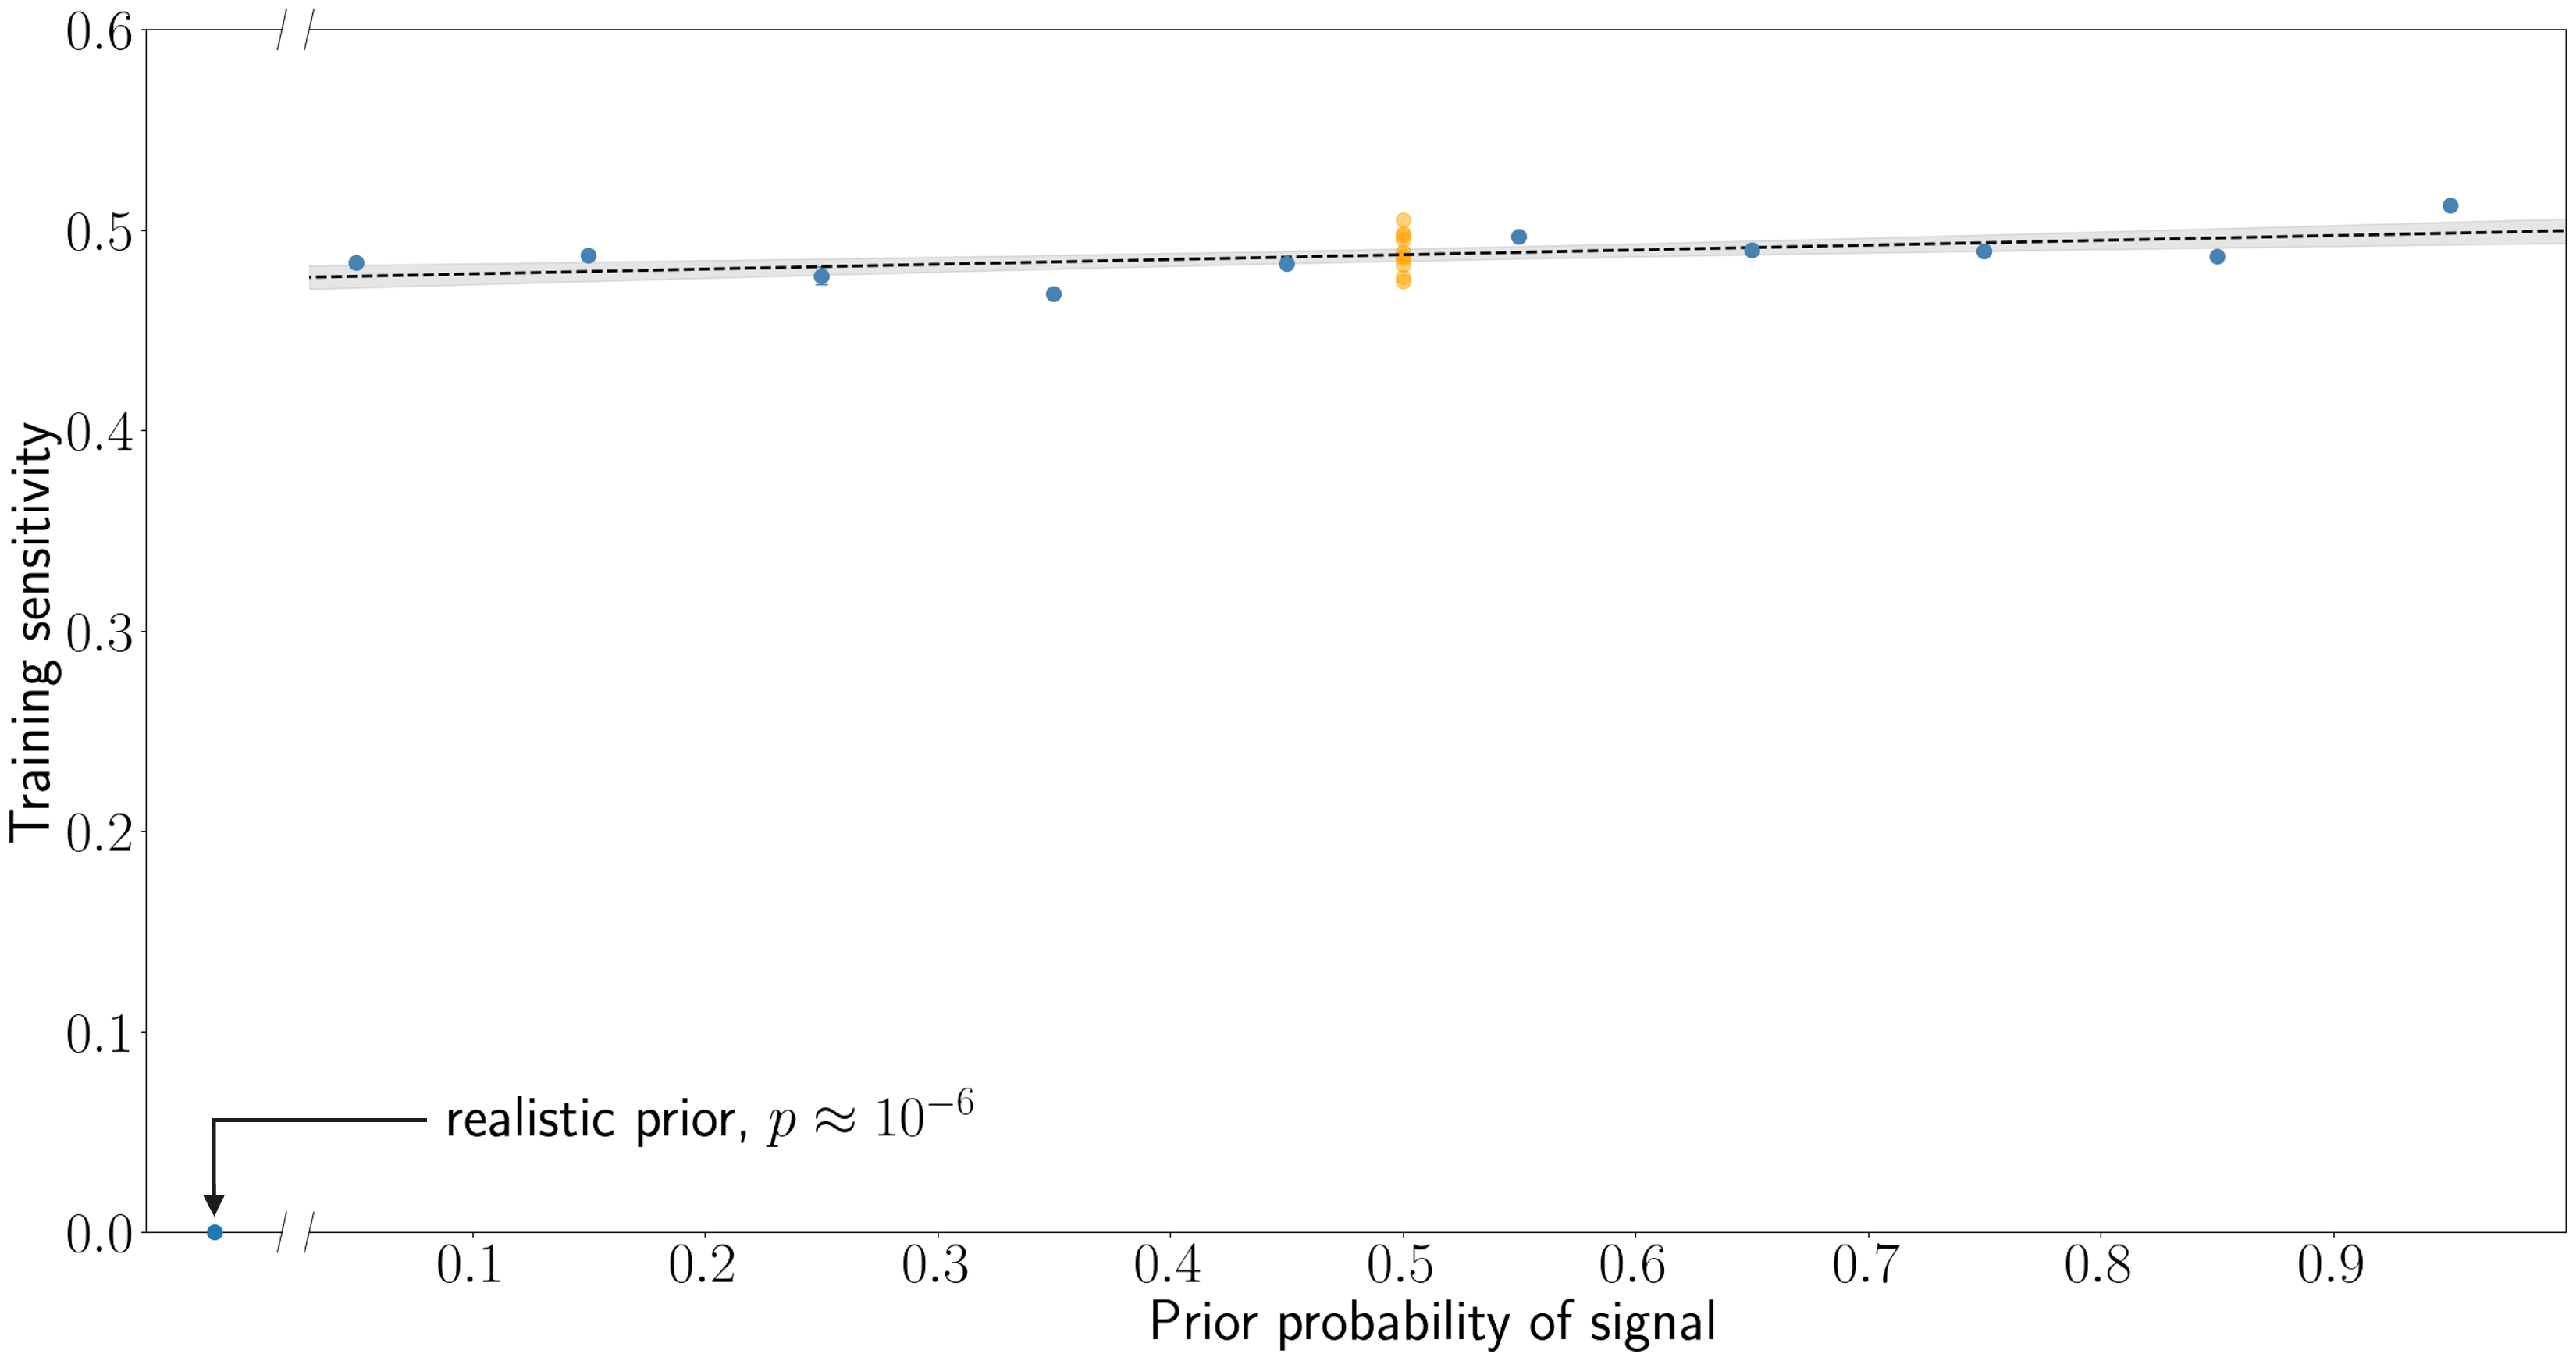
\includegraphics[width=0.9\textwidth]{./plots/prior_discussion}
	\caption{A very faint positive slope ($m = 0.02\pm0.01$) is observed when relating prior probability to trigger sensitivity (blue dots) of an example 
	convolutional neural network with the architecture in \autoref{ssec:cnn-architecture}. A charge cut of $t_S = \SI{0.5}{\Charge}$ is applied for signal 
	labelling. The observed fluctuations could however be attributed to statistics in the training fit. An ensemble of networks with the same architecture trained
	on the same data and with a single prior shows a comparable spread (orange dots).}
	\label{fig:prior-discussion}
\end{figure}

\subsection{Further hyperparameters}
\label{ssec:further-hyperparameters}

The number of ways both input data and the network architecture can be tweaked to minimize loss is extensive. Further optimization methods, like the choice of 
labelling, are motivated and discussed in the performance reports in \autoref{sec:cnn-performance}.

One promising approach of optimizing trigger performance that is not examined in this thesis is the adjustment of the neural network loss function. Several reasons
exist that motivate an analysis in this direction:

\begin{itemize}
	\item \textbf{Classwise weighting:} The classes $\mathcal{C}_1$ and $\mathcal{C}_2$ are seen as equally important when calculating efficiencies by default. 
	As noted in \autoref{ssec:input-data} an imbalance in distributions exists. Observing background is much more likely than observing an air shower. The loss 
	function will reflect this to an extent if classification of background is weighted more heavily than classification of signal. Even a more complex loss 
	sensitive to CR flux (compare \autoref{eq:statistics-efficiency}) or other parameters is possible.
	\item \textbf{Random-trace trigger rate pull term:} For the most part, the analysis presented here will introduce a neural network distinguished by some 
	feature, optimize its performance, and check whether the resulting random-trace trigger rate is in an acceptable range. However, it is possible to go the 
	opposite way and specify a target trigger rate first and then train the network. In this fashion, one could hope that the algorithm efficiency is optimized for
	a given bandwidth by adding a pull term to the loss function. The challenge of this approach is weighting the pull term in a way that it does not dominate the 
	loss function in different fringe cases. An important drawback of this method is that training will be very slow.
\end{itemize}

\subsection{Training procedure}
\label{ssec:training-procedure}

In order to make informed statements about the capability of a given network architecture, an ensemble of 10 networks are trained - unless specified otherwise - for 
10 epochs. Per epoch, 80\% of the available showers are examined to calculate gradients, the remaining 20\% are set aside for validation purposes. This is a standard 
procedure to prevent the network from overfitting training data \cite{nasteski2017overview}. Since the training dataset is extensive ($0.8\cdot40557\approx32445$ 
showers), convergence to a local minimum is typically observed already within a single epoch. For this purpose, training is halted early if the training accuracy
is greater than $\alpha = 0.95$ and no decrease in loss has been observed for at least $75\%\,\hat{=}\,24334\;\text{showers}$ of the epoch

\section{CNN Trigger}
\label{sec:cnn-performance}

\subsection{Architecture}
\label{ssec:cnn-architecture}

The convolutional neural networks presented in this chapter all have a very similar architecture, which was shown to slightly outperform other candidates during 
prototyping tests. It is likely that this is due to design ideas that are closely related to the way information is structured in the time traces:

\begin{itemize}
	\item A \textbf{2D convolutional input layer} (c.f. \autoref{sec:CNN}) pools together the information of the three different WCD PMTs.
	\item A \textbf{1D convolutional layer} resolves temporal correlation in the output of the previous layer.
	\item A \textbf{Dense layer} reduces the extracted features to a binary choice of signal and background.
\end{itemize}

In subsequent tests, it is furthermore concluded that extending the architecture by an intermediate dense layer between the time convolution layer and the dense 
output layer is on average beneficial for signal to noise ratio. However, because both approaches arrive at a similar best score, the smaller, non-extended network
is seen as more viable for the use case in the Pierre Auger Observatory. An example performance of both models is given in \autoref{fig:cnn-vs-ecnn}. The 
corresponding number of trainable parameters is given in \autoref{tab:network-parameters}. The precise implementation designs for both cases are shown in 
\autoref{fig:cnn-architecture}.

\begin{figure}
	\centering
	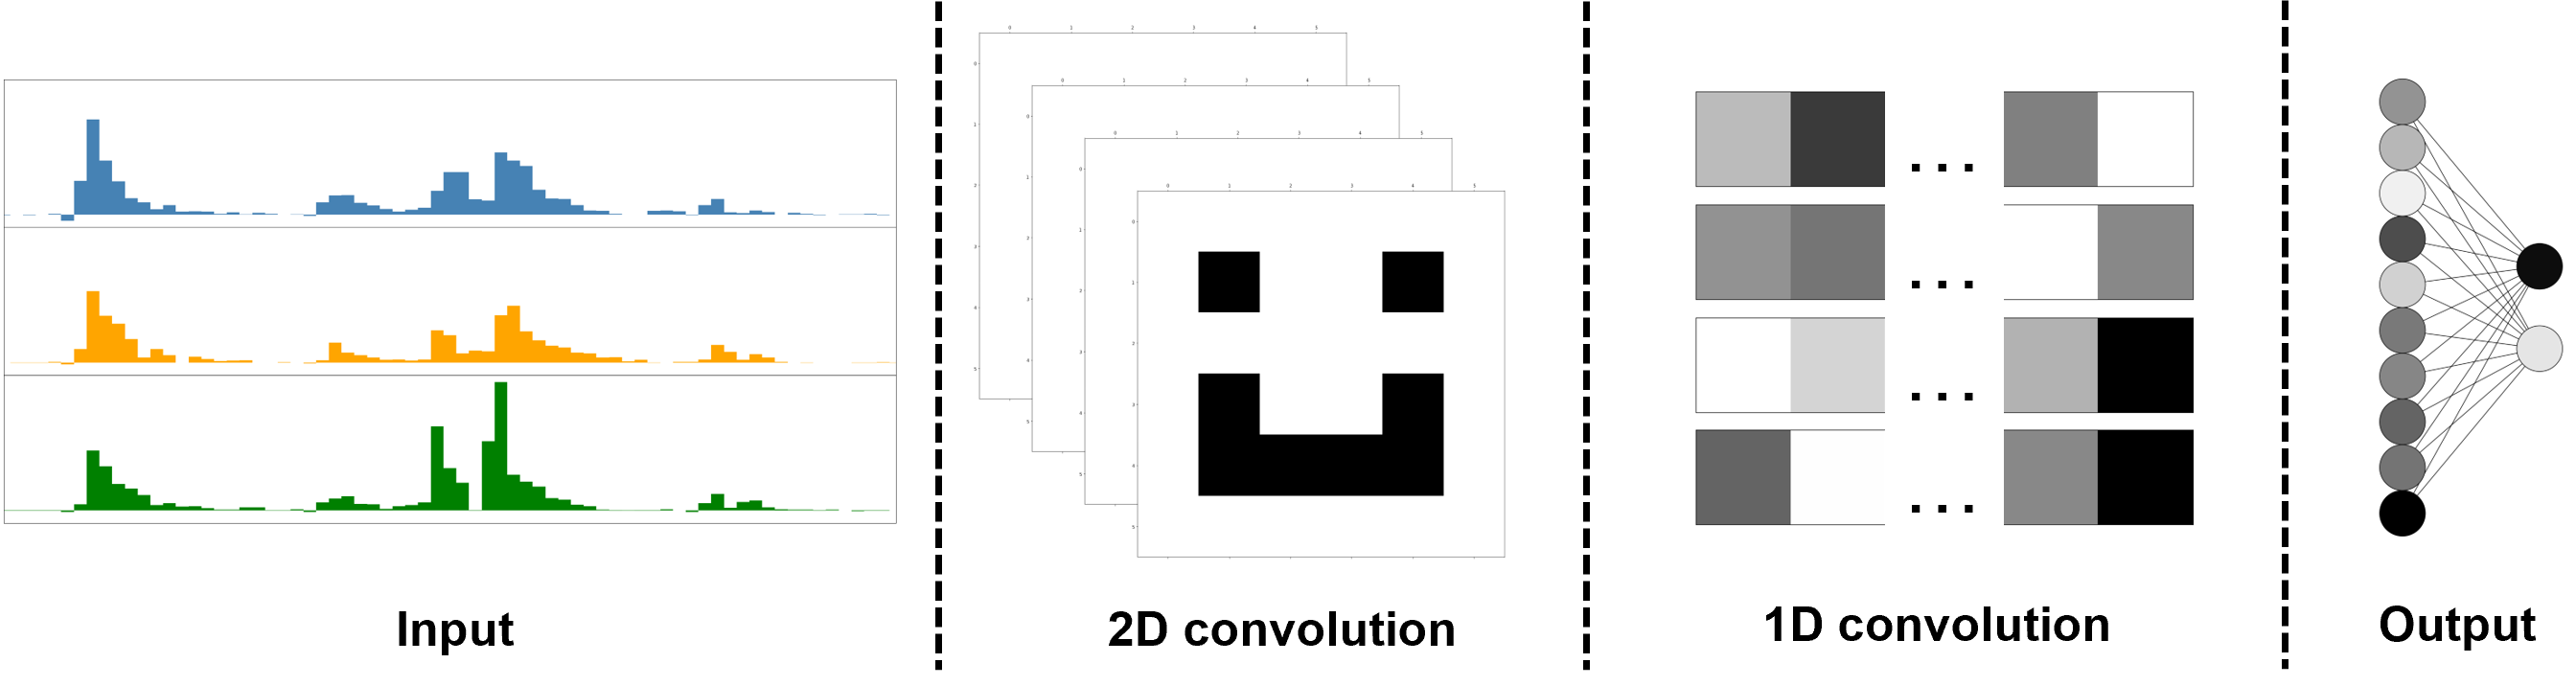
\includegraphics[width=0.9\textwidth]{./imgs/CNN_architecture.png}
	\caption{The convolutional neural networks take a two-dimensional input consisting of a time trace excerpt of the three WCD PMTs. On this input data, a 
	two-dimensional convolution is performed with four different filters, resulting in four one-dimensional vectors that are propagated further. A one-dimensional
	convolutional layer scans the previous outputs and extracts two features per vector, these are finally reduced to a binary output via a dense layer with 
	softmax activation. For extended CNNs, a dense layer with 10 neurons is interposed with a relu activation function.}
	\label{fig:cnn-architecture}
\end{figure}

\begin{table}[h]
	\begin{center}
	\caption{Number of training parameters $n_\text{Train}$ for different network architectures}
	\begin{tabular*}{0.8\textwidth}{@{\extracolsep{\fill}} ccccc}
		\toprule
		Type & Input size & Kernel size & $n_\text{train}$ & w/ dense extension \\
		\midrule
		CNN & $(3, 120)$ & $(3, 3)$ & $\mathbf{140}$ & $\mathbf{834}$ \\
		CNN & $(3, 120)$ & $(3, 10)$ & $\mathbf{216}$ & $\mathbf{534}$ \\
		CNN & $(3, 120)$ & $(3, 30)$ & $\mathbf{444}$ & $\mathbf{714}$ \\
		CNN & $(3, 40)$ & $(3, 3)$ & $\mathbf{84}$ & $\mathbf{210}$ \\
		CNN & $(3, 60)$ & $(3, 3)$ & $\mathbf{100}$ & $\mathbf{290}$ \\
		CNN & $(3, 90)$ & $(3, 3)$ & $\mathbf{120}$ & $\mathbf{390}$ \\
		CNN & $(3, 240)$ & $(3, 3)$ & $\mathbf{220}$ & $\mathbf{890}$ \\
		LSTM & $(3, 120)$ & $-$ & $\mathbf{12}$ & (single layer) \\
		LSTM & $(3, 120)$ & $-$ & (three layers) & $\mathbf{44}$ \\
		\bottomrule
	\label{tab:network-parameters}
	\end{tabular*}
	\end{center}
\end{table}

\begin{figure}
	\centering
	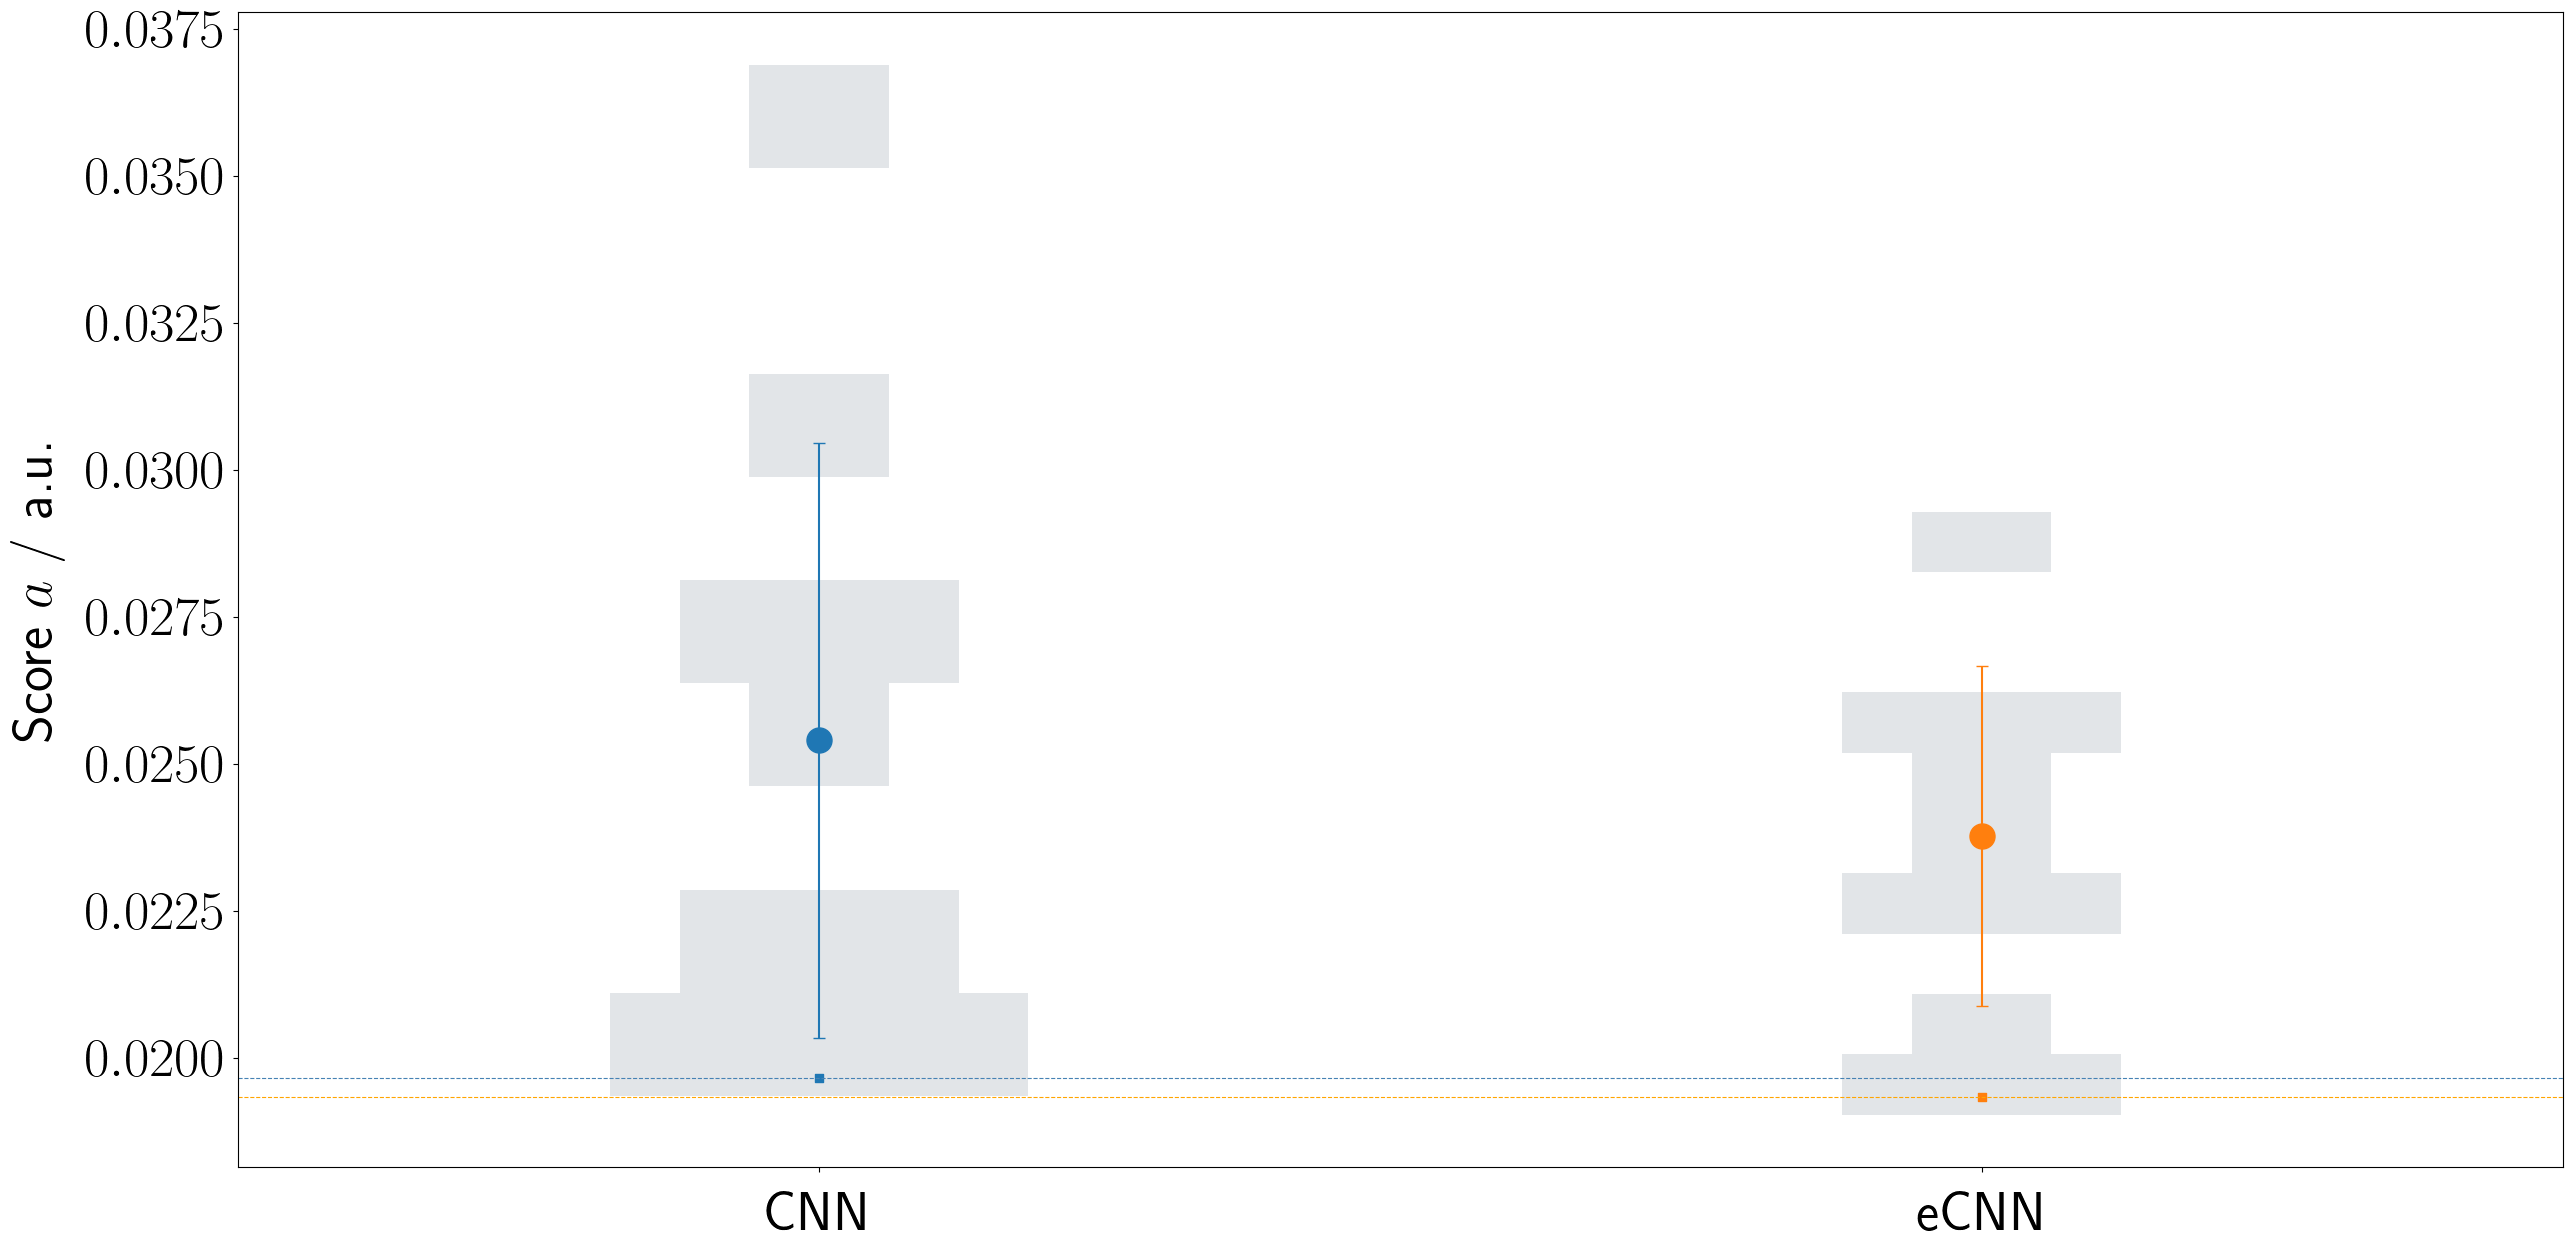
\includegraphics[width=0.9\textwidth]{./plots/CNN_vs_eCNN.png}
	\caption{The network score as calculated in \autoref{eq:comparison-score} is compared from original network architecture (CNN, left, in blue) to the extended
	architecture featuring an additional dense layer (eCNN, right, in orange). Shown are 10 networks of each architecture trained on the same dataset. Both
	architectures find a similar best solution (squares), while the mean and spread of the population (circles) are smaller for the extended network.}
	\label{fig:cnn-vs-ecnn}
\end{figure}

\subsection{Performance}

Training a convolutional neural network with the data from \autoref{chap:neural-network-data} as is results in near perfect accuracy. The lateral trigger 
probability obtained after training is equal to the LPP (see \autoref{fig:NN-LPP} and \autoref{fig:lateral-particle-probability}), which quantifies the probability
of particle existance at station level. This implies that the networks are able to identify even single particles in the WCD with very high confidence. However, 
they have not learned to distinguish muonic events from actual extensive air showers. This results in a very high random-trace trigger rate of 
$f_\text{Random} > \SI{2}{\kilo\hertz}$. In order to decrease this value, the training data must be altered.

\begin{figure}
	\centering
	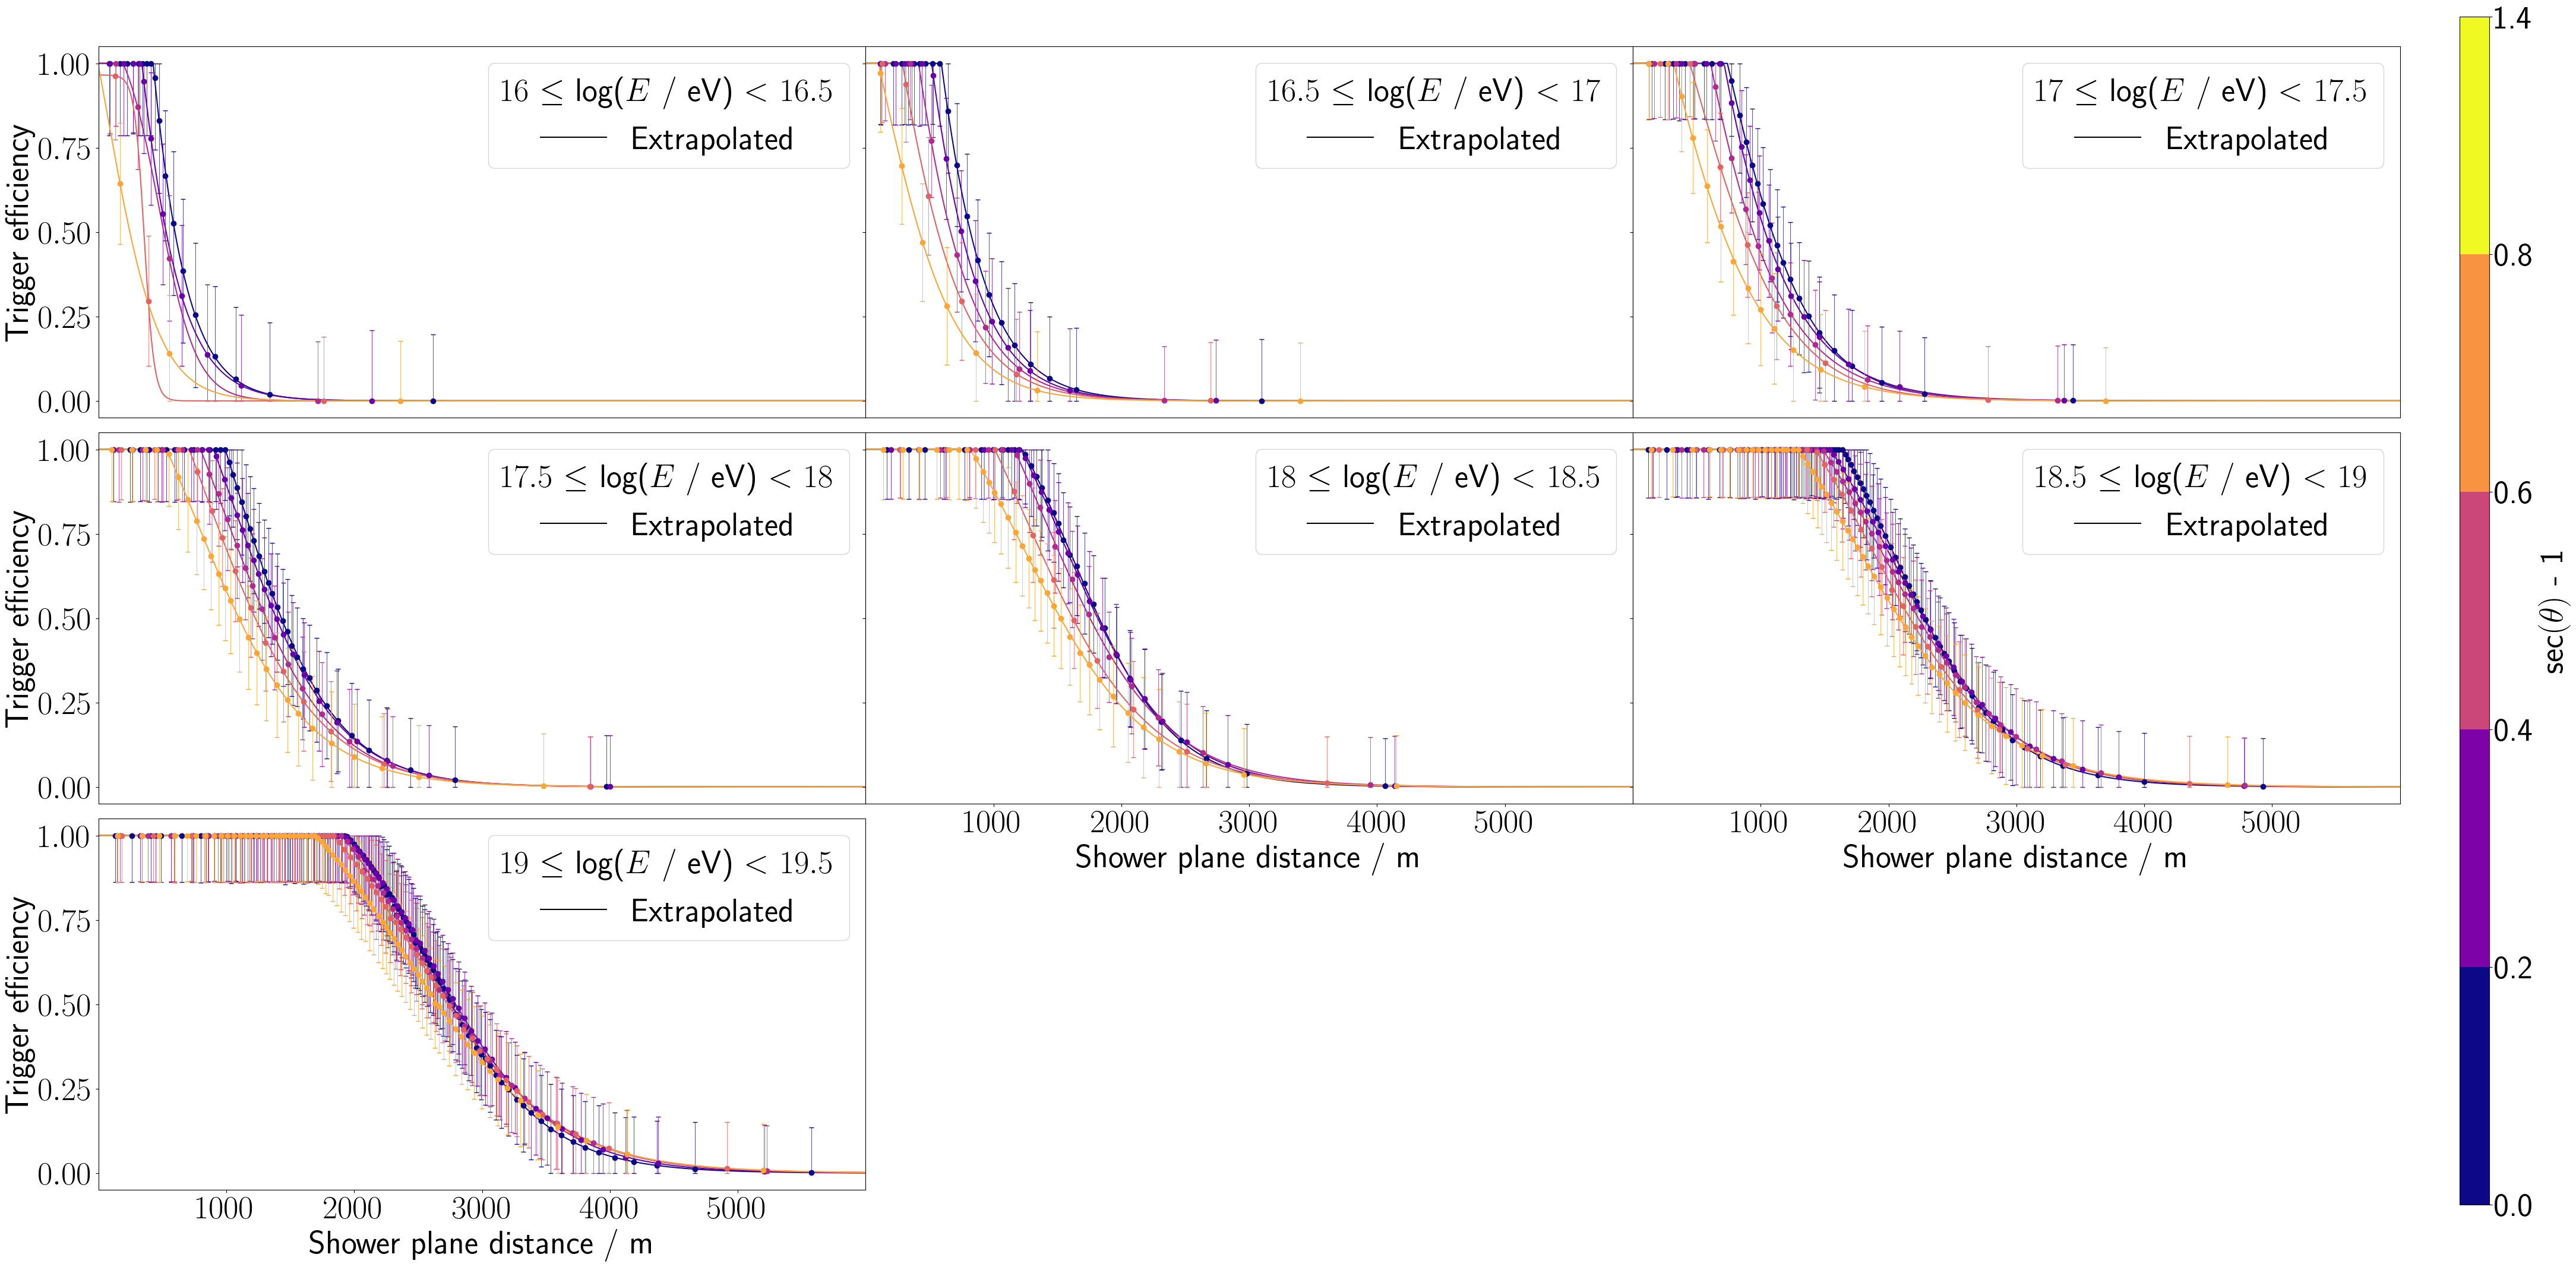
\includegraphics[width=1\textwidth]{./plots/ideal_classifier_LTP.png}
	\caption{The lateral trigger probability is equal to the lateral particle probability shown in \autoref{fig:lateral-particle-probability} for almost all 
	$E$ and $\theta$. Discrepancies occur at low primary energies and high inclinations due to low statistics complicating the LTP fit. In any case, this implies 
	that the chance of raising a T2 provided a station was hit by an air shower is 1.}
	\label{fig:NN-LPP}
\end{figure}

\subsubsection{Muon cut}

As discussed in \autoref{chap:neural-network-data}, atmospheric muons from very low-energy showers represent the dominant background (that is not just electronic 
noise) in measured data. The most straight forward approach of lowering the network sensitivity for such signals is requiring muonic coincidences. This means only 
data from tanks which were hit by at least 2, 3, ..., $n_\mu$ muons are assigned a signal label, where $n_\mu$ is a tweakable hyperparameter. Traces can be 
selected based on other particles as well. \Offline saves the number of muons, electrons and photons for simulated stations. All three, or even a (weighted) sum
are candidate discriminators. In this work, only the muon cut is analyzed with greater detail in \autoref{ssec:cnn-muon-cut}, as it is thought to be more closely 
tied to the problem of distinguishing signal from background.

Several ensembles are trained with different $n_\mu$ to test the quality of this cut. Their subsequent performance is shown in \autoref{fig:CNN-muon-cut}. The 
results are inconclusive. While low cut thresholds requiring a coincidence of $\gtrsim 2$ muons seem to represent a solid way of lowering $f_\text{Random}$, the 
trigger rates are not brought down to acceptable levels by this cut alone. Even worse, the training fits do not converge uniquely at higher cut thresholds.
This indicates the number of muons is not (at least at higher muon counts) a great discriminator. This may be attributed to several reasons:

\begin{itemize}
	\item \textbf{Lack of strict temporal coincidence}: The imposed cut only requires at least $n_\mu$ muons to hit the tank at some point during a shower event. 
	Without a more stringent requirement it is possible that a network sees not a trace stemming from $n_\mu$ muons, but rather $n_\mu$ traces from 
	individual particles during a sliding window analysis. Since all of these fit the cut criterion and are hence labelled as signal, the network does not learn
	to ignore such traces.
	\item \textbf{Variety in single muon traces}: The detector response to a single muon varies based on muon inclination, detector specifics and statistics. All
	of these are parameters that are not available to the CNN. The combination of all fluctuations might be too complex for a convolutional neural network with 
	limited size to learn.
\end{itemize}

Nevertheless, a hybrid cut requiring at least 2 muons in a tank on top of some other trace characteristic might hold potential in further analysis. A muon cut by
itself is shown to not work ideally for the data at hand.

\begin{figure}
	\centering
	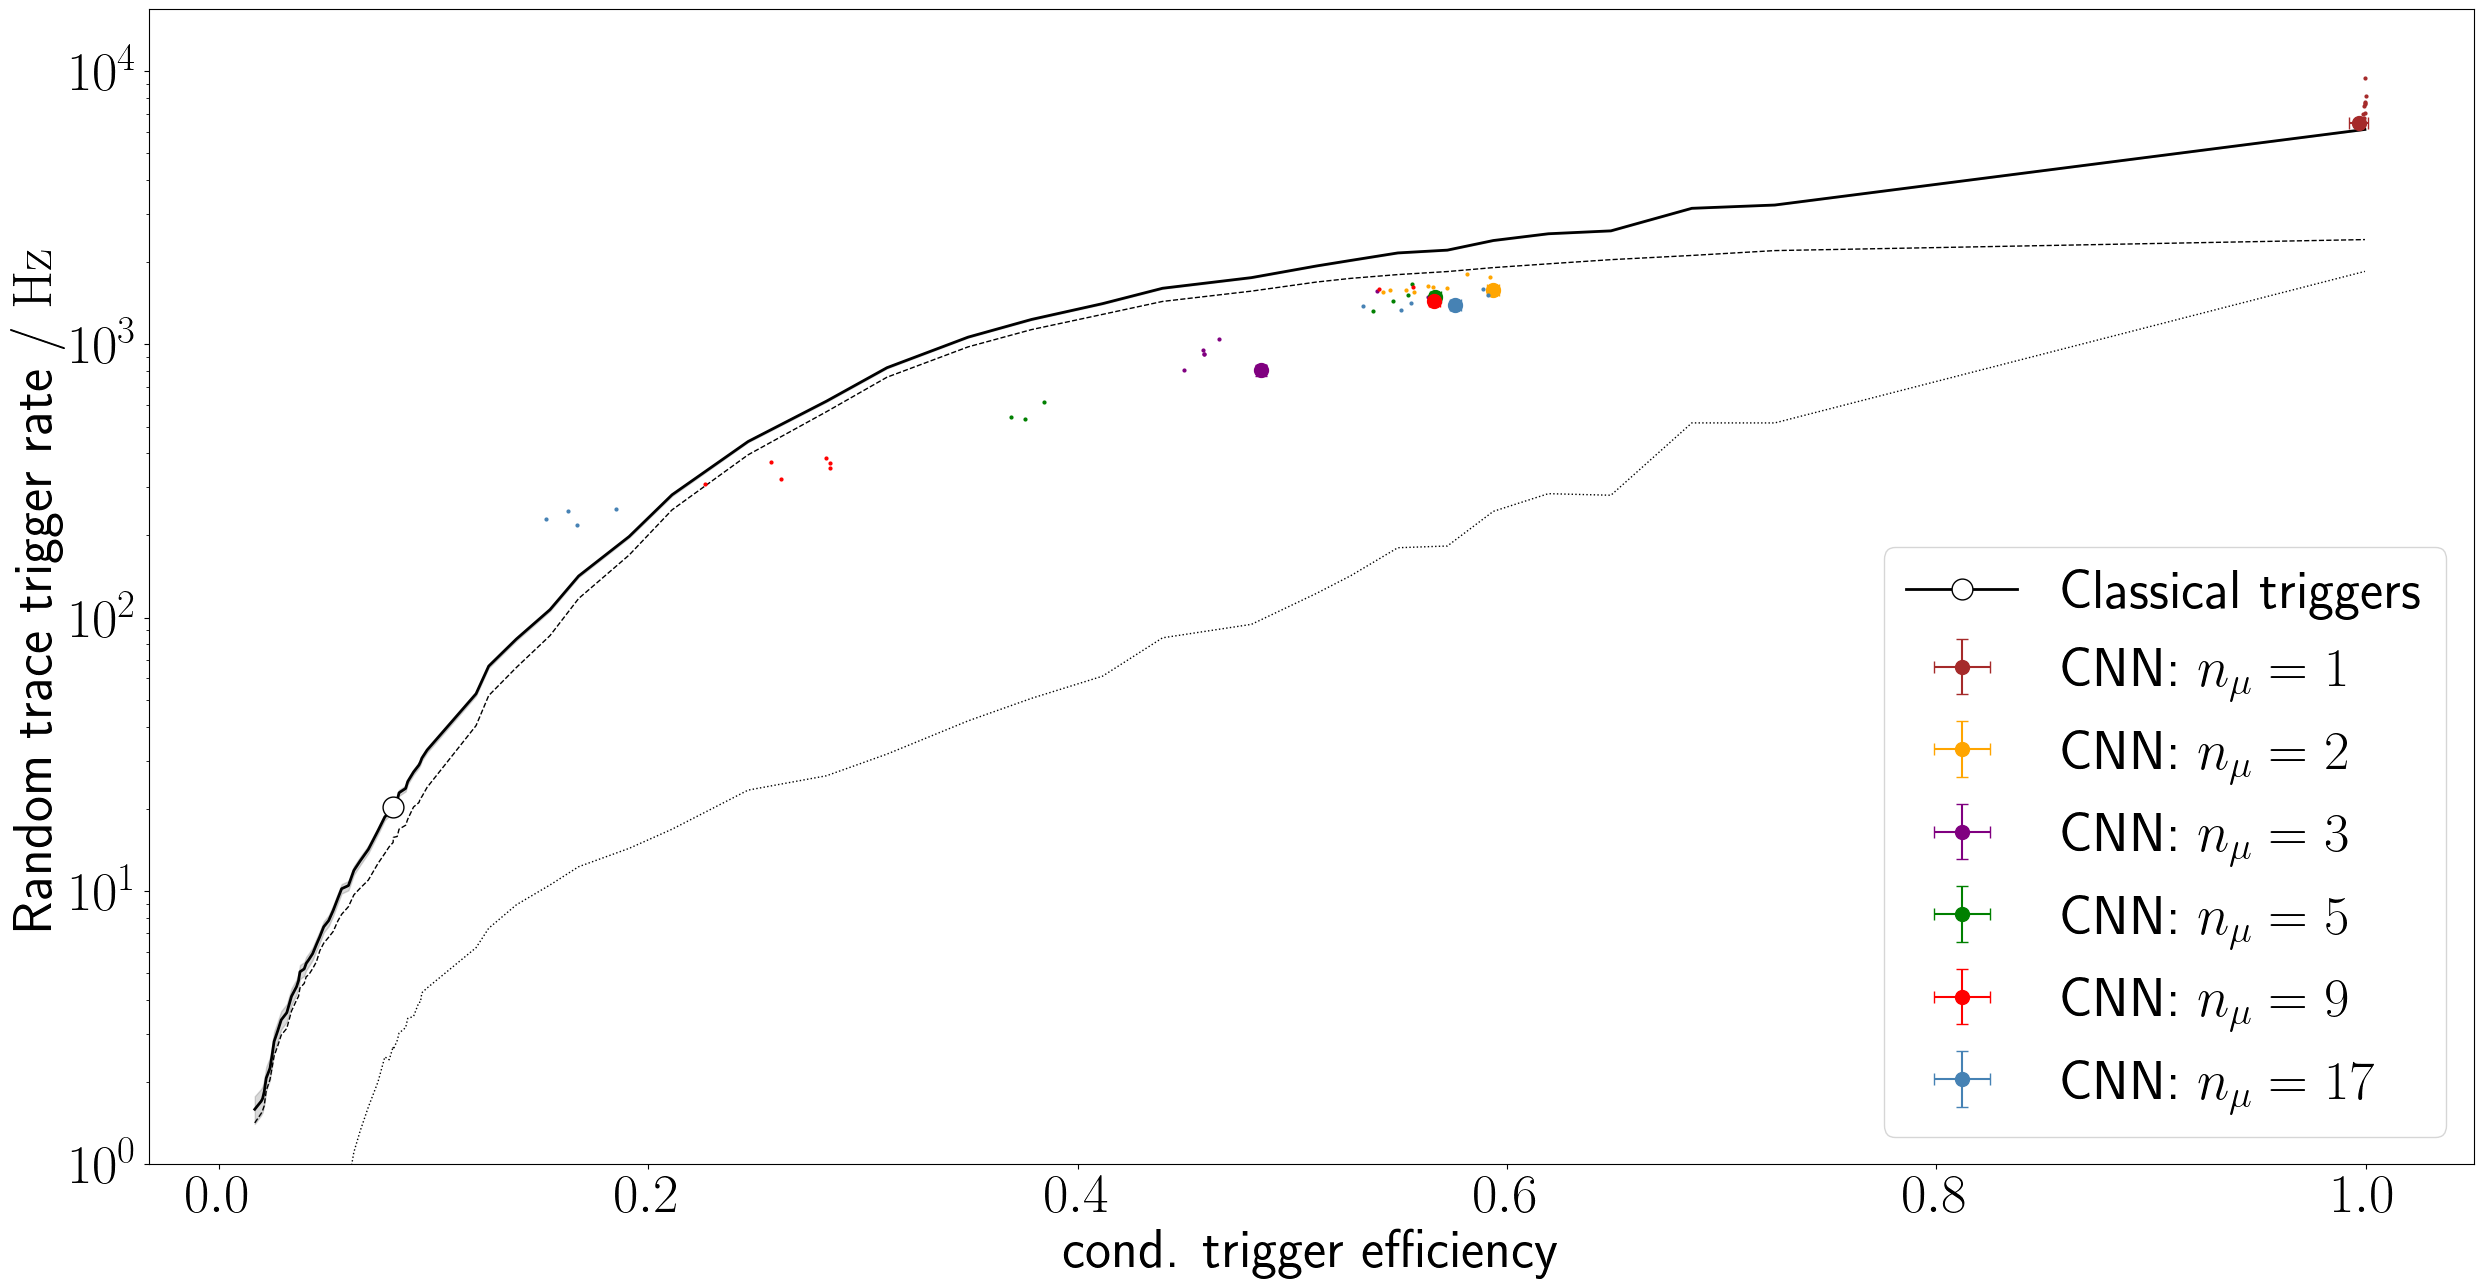
\includegraphics[width=0.9\textwidth]{./plots/CNN_muon_cut.png}
	\caption{Relation between random-trace trigger rate (lower is better) and conditional trigger efficiency (higher is better). The performance of convolutional 
	neural networks trained on data with a muon cut of different thresholds. The optimizers don't seem to identify a unique local minimum at very high cut 
	thresholds. For all intermediate cuts $1 < n_\mu < 17$ the convolutional neural networks offer a better trigger efficiency compared to the Th-T2 trigger at the
	same random-trace trigger rate. The performance of the ToT trigger is not reached.}
	\label{fig:CNN-muon-cut}
\end{figure}

\subsubsection{Charge cut}
\label{sssec:charge-cut}

Another method of teaching a network to ignore certain signals is given by imposing a cut $t_S$ on the integral $S$ of the trace. One advantage of this approach is
the fact that the choice of labelling in this case is fully determined by the input data. Another edge is the granularity of the cut. Whereas only integer values 
of $n_\mu$ are sensible in the previous paragraph, the integral is discretized in much smaller steps of $\SI[per-mode=power]{1}{\per\Charge}$. This allows for 
finer tuning of the network performance.

By increasing $t_S$, the network will learn to ignore increasingly larger signal. This is shown in \autoref{fig:CNN-charge-tpr}. The performance arising from 
different $t_S$ is shown in \autoref{fig:CNN-charge-cut}.

\begin{figure}
	\centering
	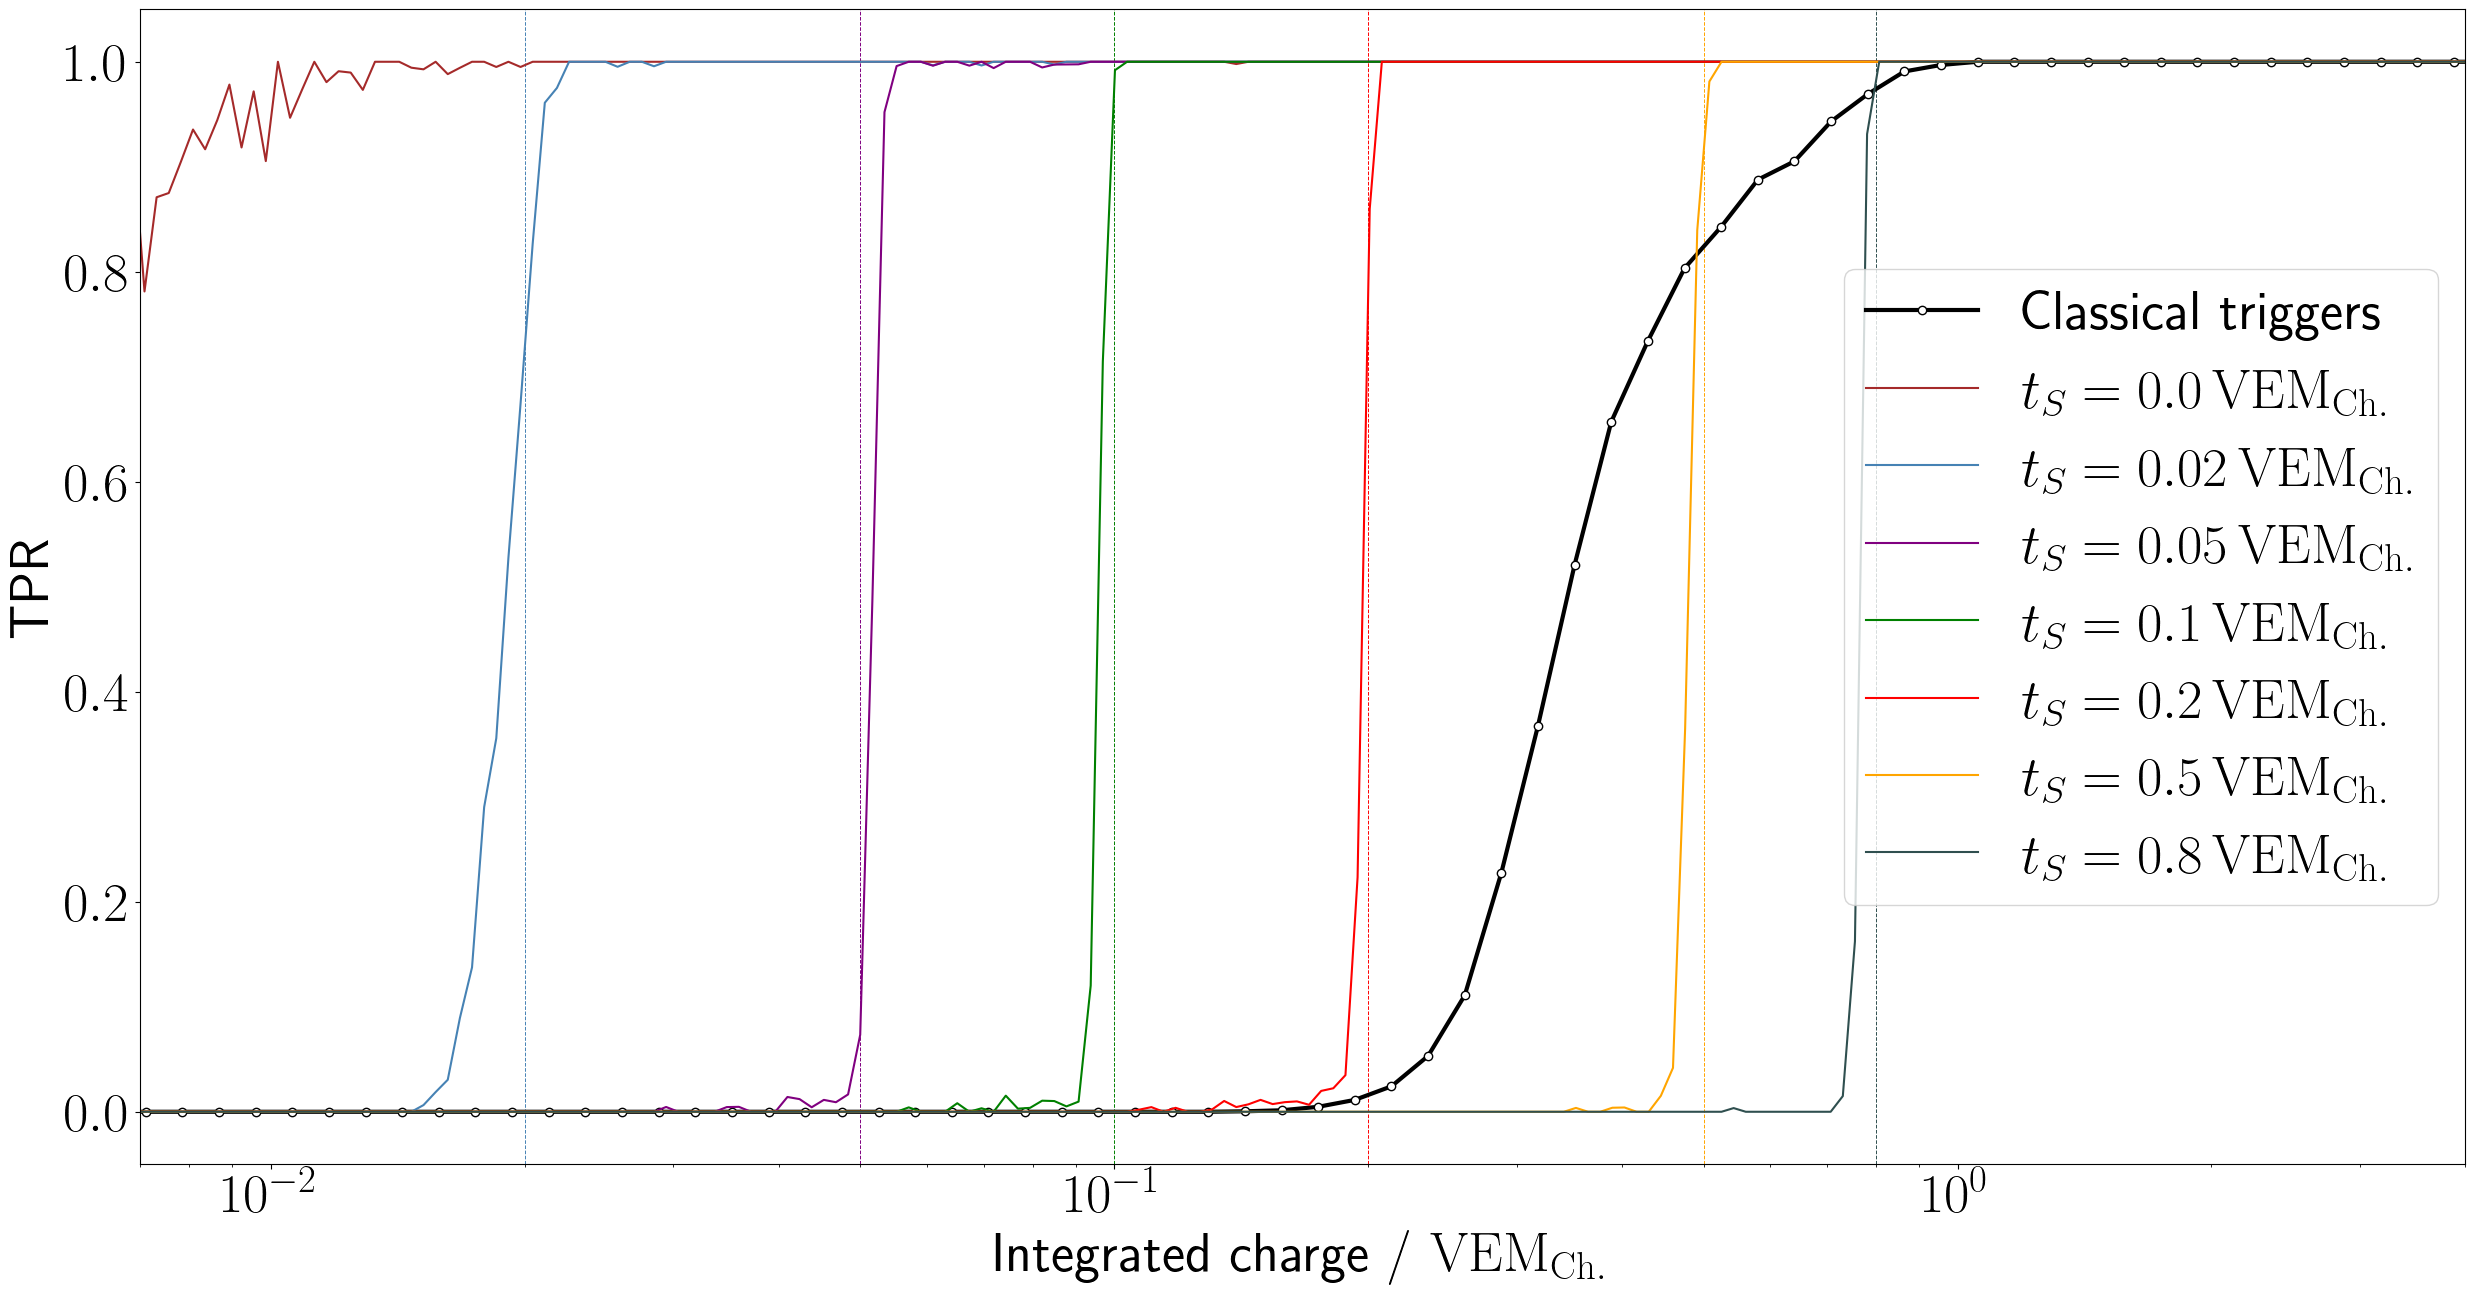
\includegraphics[width=0.9\textwidth]{./plots/CNN_charge_TPR.png}
	\caption{The true positive rate (TPR) in terms of deposited signal for different classifiers. Convolutional neural networks that were trained with a cut 
	threshold of $t_S$ will not trigger on traces that have a lower integral $t_S > S$, dropping the sensitivity in this region. This is precisely the desired 
	effect. Classical triggers become fully efficient at around $\SI{1}{\Charge}$.}
	\label{fig:CNN-charge-tpr}
\end{figure}

\begin{figure}
	\centering
	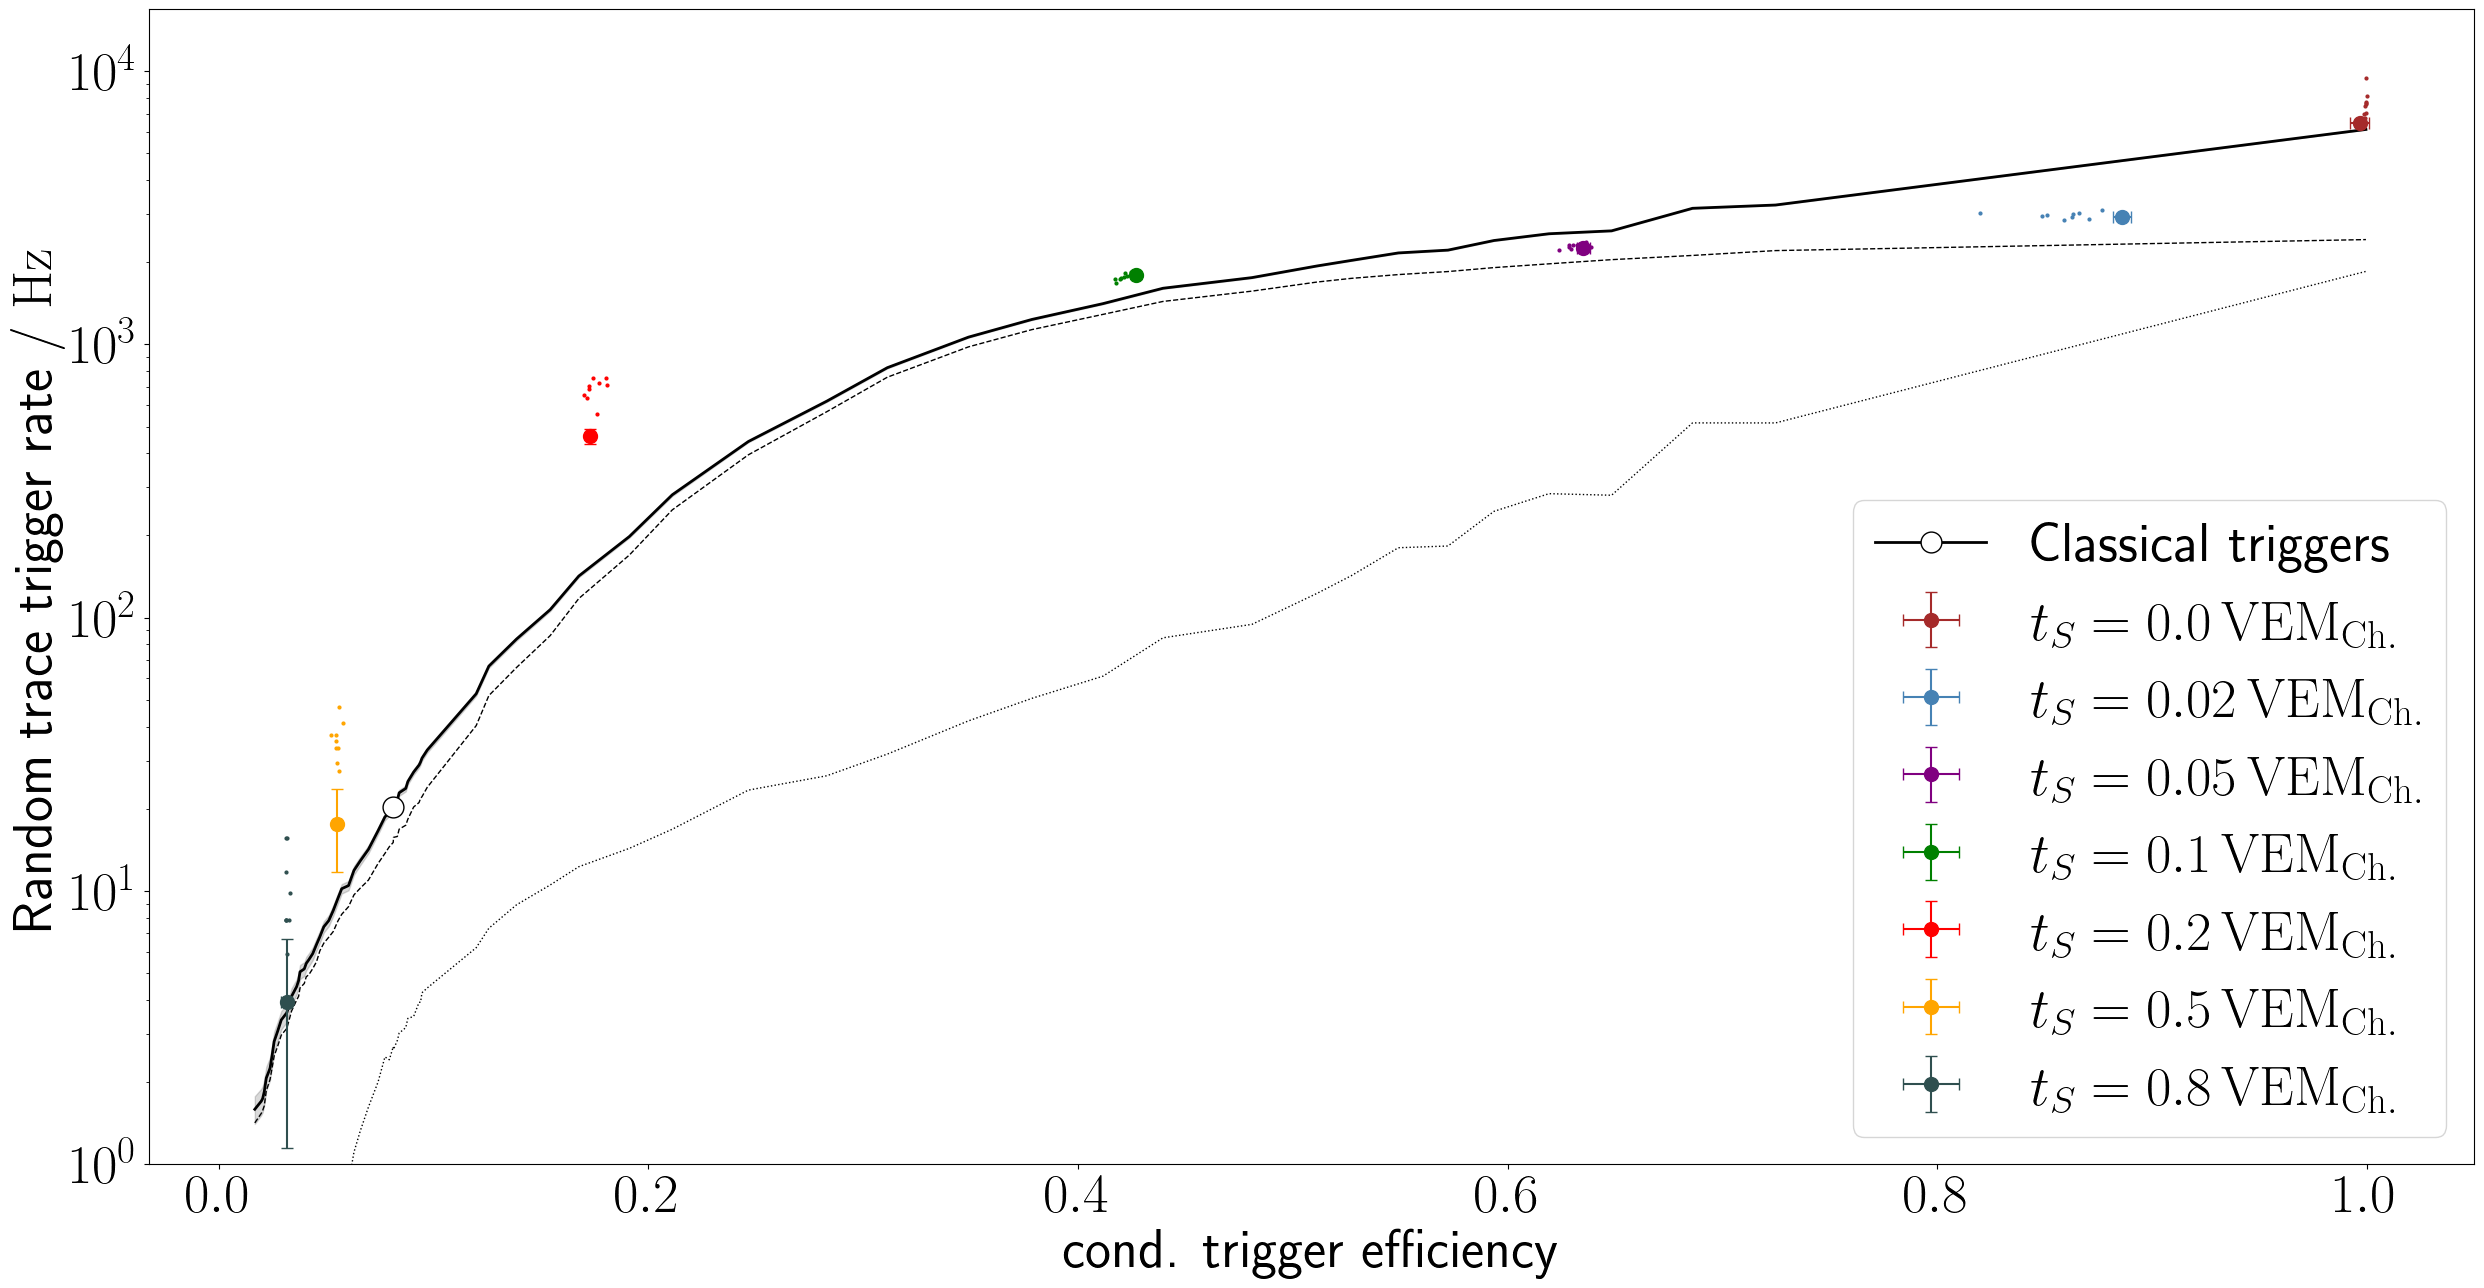
\includegraphics[width=0.9\textwidth]{./plots/CNN_charge_cut.png}
	\caption{Relation between random-trace trigger rate (lower is better) and conditional trigger efficiency (higher is better). Convolutional neural network 
	performance in relation to different integral thresholds. With an increasingly stringent cut, the networks learn to ignore more and more low-energy events, 
	which quickly drops the trigger efficiency. On the other hand, the classifiers random-trace trigger rate drops to more acceptable levels.}
	\label{fig:CNN-charge-cut}
\end{figure}

\subsubsection{Full Bandwidth vs. Filtering \& Downsampling}
\label{sssec:full-bandwidth-filtering-downsampling}

Charge cutting provides a powerful method to control the conservativity of the classifier and force discrimination between muonic background and extensive air 
showers. Equipped with this tool, other questions can be answered in an attempt to optimize network performance.

For example, classical triggers are run in compatibility mode, where 3 UUB bins (\SI{8.3}{\nano\second}) are filtered and downsampled to resemble a single UB bin 
(\SI{25}{\nano\second}). Some information about the trace shape is lost in the process. Logically, a neural network should be able to identify original UUB signal 
traces with more ease than their filtered and downsampled counterparts. Ideal triggers should have a higher efficiency when tested on full bandwidth traces.

This does not render compatibility mode uninteresting for analysis. An effective way of minimizing the trainable parameters in a neural network is reducing its' 
number of input parameters. Filtering and downsampling encodes - albeit imperfectly - the input data and reduces the dimensionality by a factor of three. This is
done in such a way that the UB-like trace contains trace information from a time window that is three times as long for a given number of bins.

Consequently, by filtering and downsampling input data it becomes possible to hand the classifiers additional information while keeping the network size at a fixed
level. The effects this has on predictive power of neural networks is shown in \autoref{fig:CNN-filtering-vs-downsampling}.

Classifiers trained on compatibility mode traces consistently have a lower random-trace trigger rate while operating at the same efficiency. Whether this is caused
by the above discussed difference in (temporal) input size or other trace characteristics is determined in the next paragraph.

\begin{figure}
	\centering
	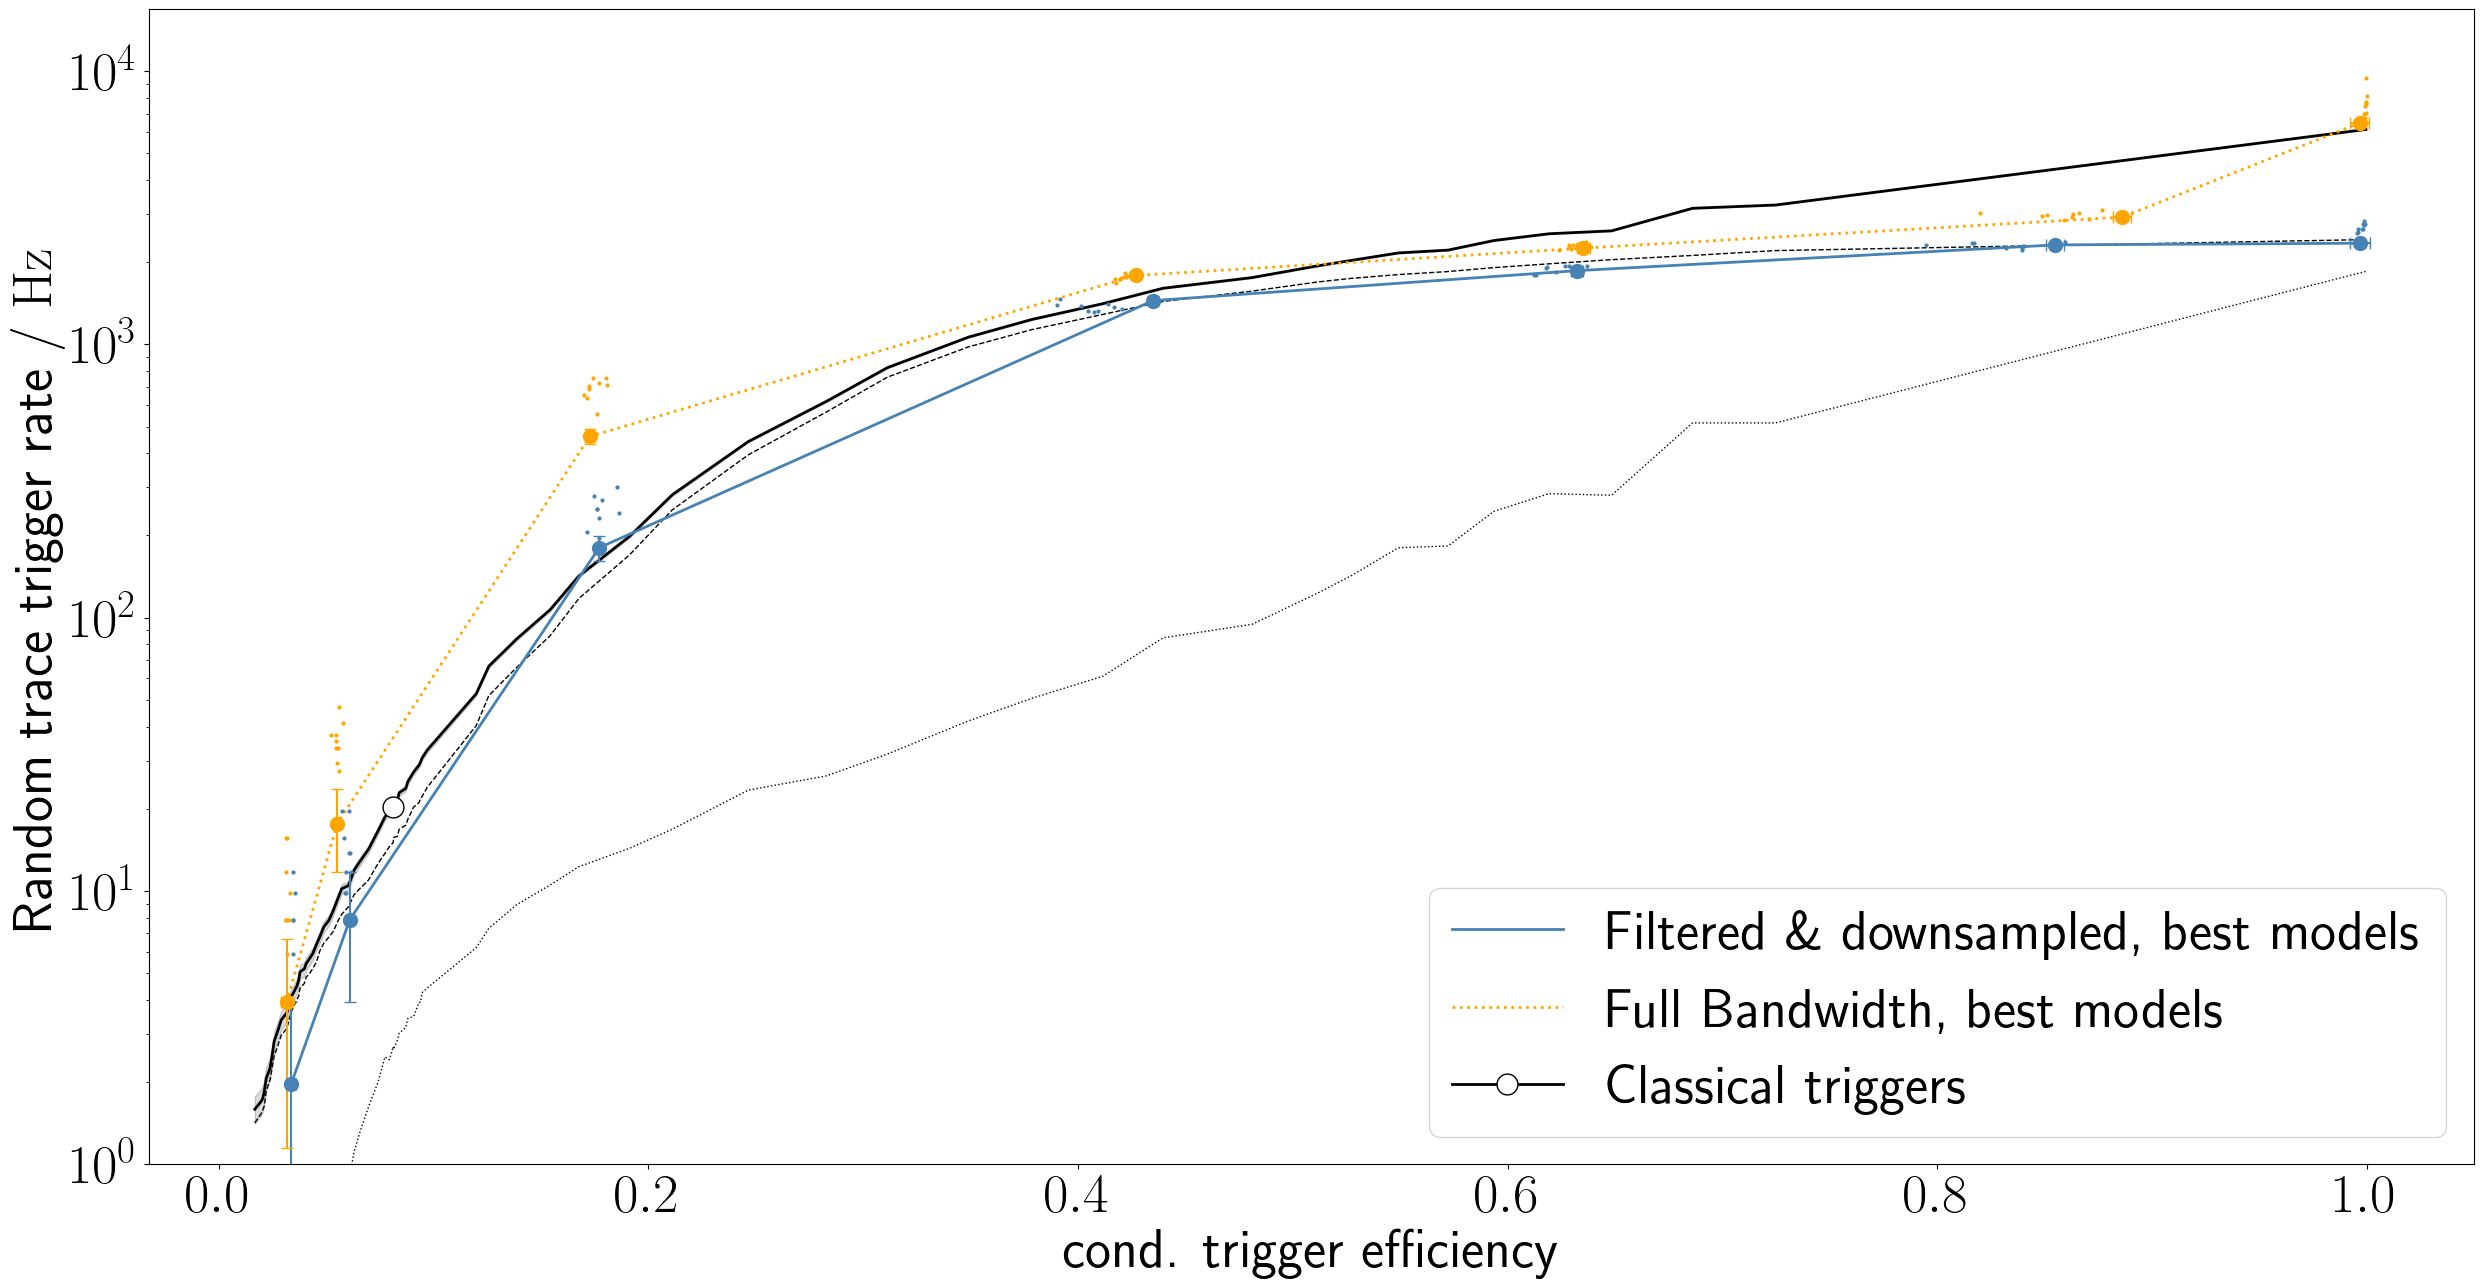
\includegraphics[width=0.9\textwidth]{./plots/full_bandwidth_vs_filtering.png}
	\caption{Relation between random-trace trigger rate (lower is better) and conditional trigger efficiency (higher is better). Convolutional neural networks 
	trained on compatibility mode traces compared to networks trained on full bandwidth traces. Compatibility-trained networks consistently have a lower random-trace 
	trigger rate}
	\label{fig:CNN-filtering-vs-downsampling}
\end{figure}

\subsubsection{Input size}
\label{sssec:input-size}

To test whether filtering and downsampling input data gives the classifiers an edge when predicting labels, multiple ensembles are trained on the same dataset with 
the same charge cut $t_S = \SI{0.5}{\Charge}$. Each ensemble differs in the size of the input trace. If compatibility-trained networks are still outperforming full 
bandwith ones that have an input size three times the size, filtering \& downsampling is the preferred method for classifying air showers with convolutional neural
networks.

Indeed, this is found. While the compared networks converge to a similar trigger efficiency, the networks that receive filtered and downsampled traces show a lower 
random-trace trigger rate. Furthermore, a larger input size slightly positively influences trigger efficiency at the cost of increased network size (c.f. 
\autoref{tab:network-parameters}). This is expected. A larger input size will result in a larger number of trainable parameters. With more trainable parameters, 
the training loss can be minimized further simply by arguments of fit dimensionality. 



\begin{figure}
	\centering
	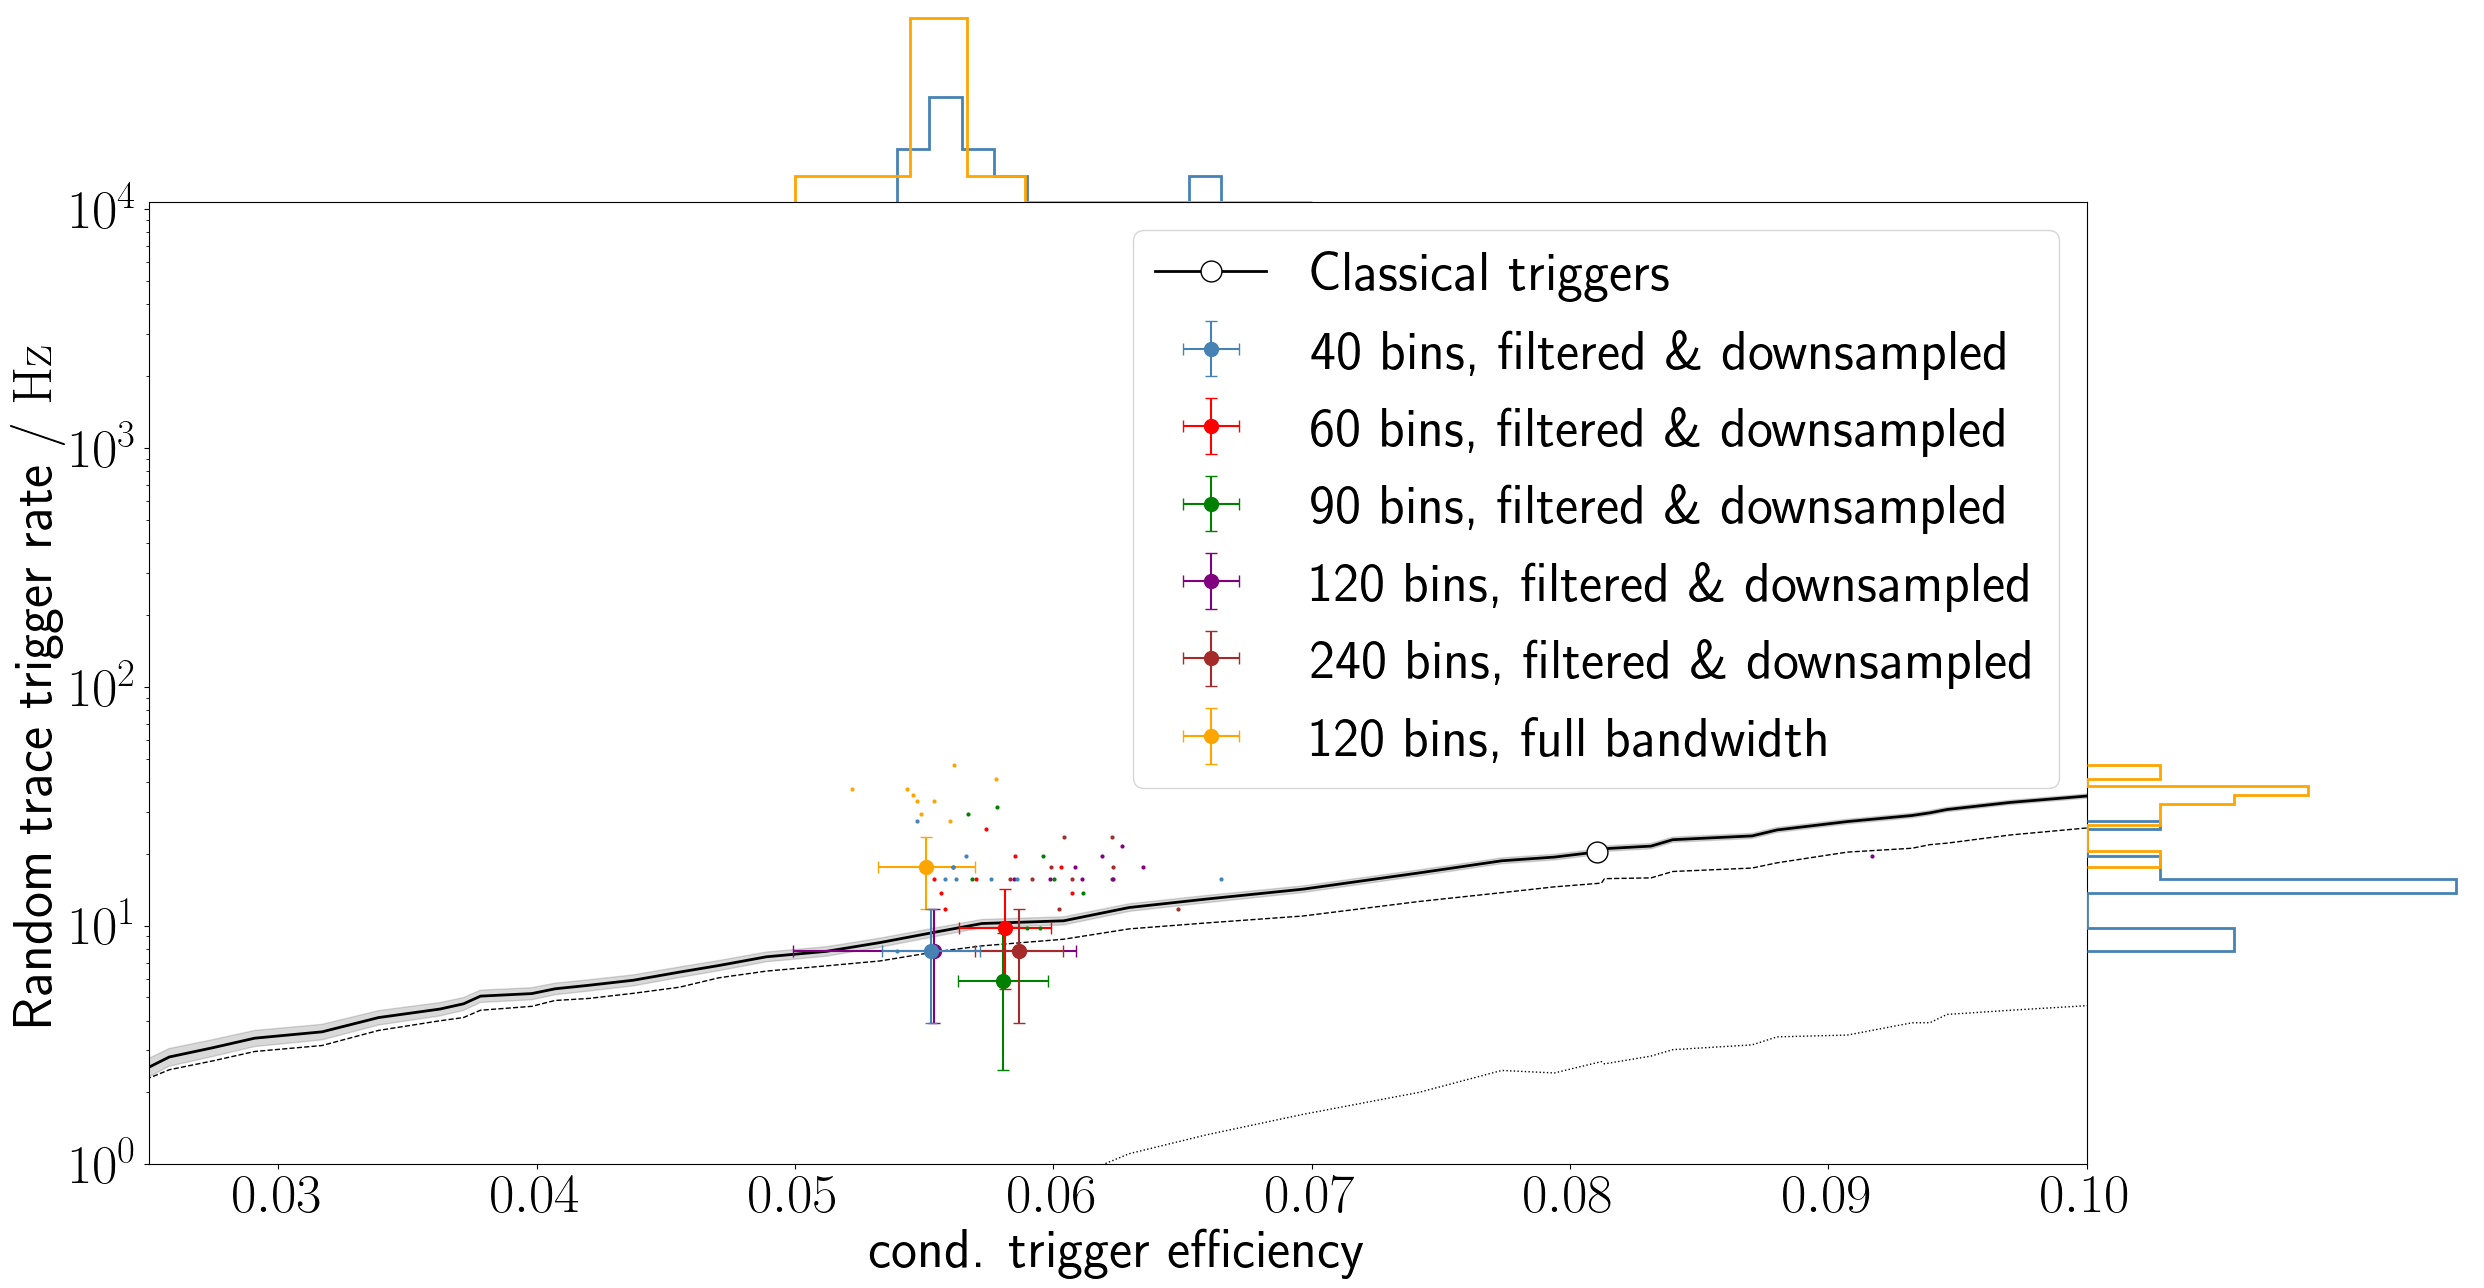
\includegraphics[width=0.9\textwidth]{./plots/CNN_input_size.png}
	\caption{Relation between random-trace trigger rate (lower is better) and conditional trigger efficiency (higher is better). The comparison between a 
	compatibility mode convolutional neural network (blue) that has the same input size in time to a full bandwidth network (orange) reveals the advantage of 
	filtering \& downsampling. Both networks have a comparable efficiency, but the compatibility mode network is less sensitive	to background triggers from 
	random-traces.}
	\label{fig:CNN-input-size}
\end{figure}

\subsubsection{Kernel size}
\label{sssec:kernel-size}

The presented models so far show a performance that is similar to the Th-T2 threshold trigger. In an attempt to boost performance, the network architecture is 
altered. Namely, the kernel size of the 2D convolutional input layer is increased. While this extends the network size, it could be expected that the 
consideration of a larger window during convolution helps the network extract more meaningful features, and increases predictive power in the process.

Three architectures are examined to check for a trend in prediction efficiency. The original $(3, 3)$-kernel only takes a minimum window into consideration. 
It has the lowest accuracy out of all models. The two other candidates have a kernel size of $(3, 10)$ and $(3, 30)$ respectively. Both have a very similar 
performance as can be seen in \autoref{fig:CNN-kernel-size}. 

Trigger efficiency is not strongly correlated to kernel size beyond a certain level. An increase in network score is not achieved by increasing it. All 
architectures have a performance very similar to the threshold trigger.

\begin{figure}
	\centering
	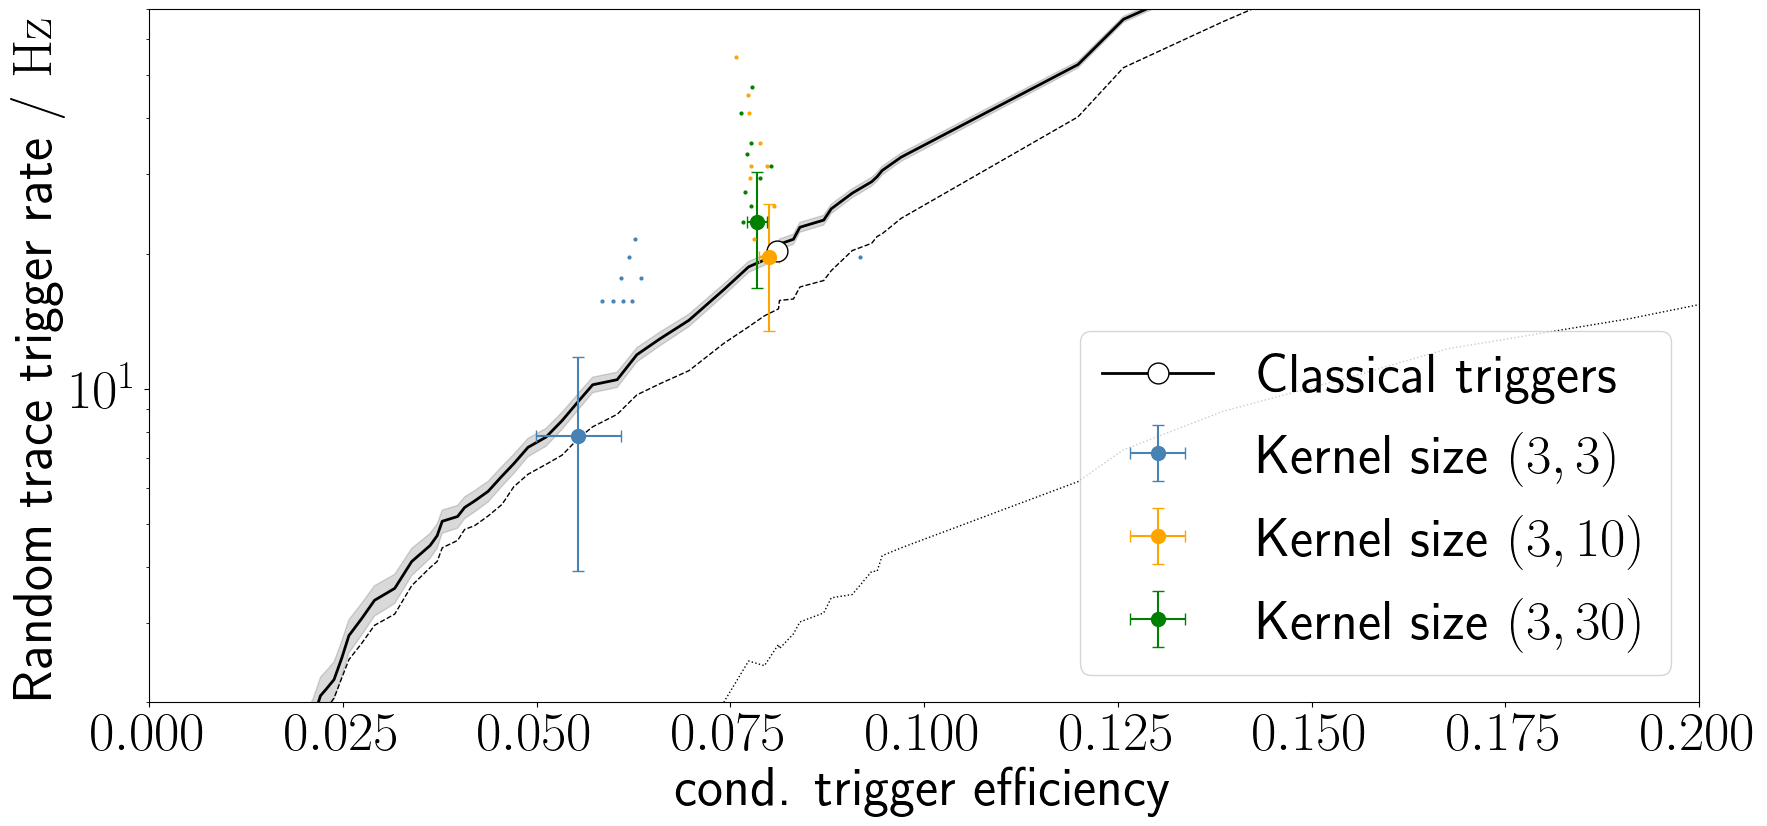
\includegraphics[width=0.9\textwidth]{./plots/CNN_kernel_size.png}
	\caption{All listed networks are trained with $t_S = \SI{0.5}{\Charge}$. An increase in kernel size benefits trigger efficiency to some extent. On the other
	hand, random-trace trigger rate increases. No clear trend in network score can be seen.}
	\label{fig:CNN-kernel-size}
\end{figure}

\section{LSTM Trigger}
\label{sec:lstm-performance}

\subsection{Architecture \& training procedure}
\label{ssec:lstm-architecture}

From \autoref{chap:neural-networks} it follows that LSTMs are especially adept at handling temporally correlated data. The deployment of RNN-based triggers thus 
seems promising for the problem at hand. The special architecture of LSTMs must however be incorporated in a larger network, as the input of an LSTM is a 
vector of single dimension, and incompatible with the data structure of a time trace. In the following, the time traces from each PMT will individually be passed
through an LSTM layer. The information extracted by the different layers will then be combined via a densely connected layer that propagates features to a binary
output representing the signal labels. This philosophy of propagating data is very similar to the ToT-like triggers, which first check trigger conditions per PMT,
and then require coincident trigger conditions for at least two PMTs (compare \autoref{ssec:threshold-trigger}).

While the chosen architectures represent very small networks ($<50$ trainable parameters, c.f. \autoref{tab:network-parameters}), calculating gradients for the 
special layout is intensive. A training step for LSTM networks takes approximately ten times as long as for CNN networks. For this purpose, the LSTMs are only 
trained for a maximum number of 5 epochs. In practice, this restriction was never needed, as the recurrent networks showed convergence after $1$ epoch already.

The hyperparameters used in training LSTMs are the ones that show the most promising results in the analysis of CNN trigger performance. Most importantly, this 
means that the input data of classifiers in this section are filtered \& downsampled.

\subsection{Performance}
\label{ssec:cnn-charge-cut}

\subsubsection{Single layer LSTM}
\label{sssec:single-layer-lsmt}

Since the arrival direction ($\theta, \phi$) is a priori random, there should be no distinguished PMT in the WCD that takes a precedent role in triggering. This 
implies that the input time trace should be treated equally whether it is coming from PMT \#1, PMT \#2, or PMT \#3. Logically, a single layer for all three input
dimensions should show the same performance as three different layers. 

This cannot be verified. An attempt to fit such an architecture to data fails. It is theorized that this is likely due to limitations of the underlaying TensorFlow 
optimization method. A subsequent analysis in the next paragraph will be conclude that no absolute ordering of layers exist, i.e. any permutation of three distinct
layers will on average arrive at the same prediction for signal or background label. With a more elaborate training setup, it is expected that a single-layer LSTM 
performs as good as a multi-layer LSTM. With a number of just 12 parameters per layer, this will drop the network size considerably.

\subsubsection{Multi layer LSTM}
\label{sssec:multi-layer-lsmt}

Using a more involved network with three distinct LSTM layers as well as dense output layer, the performance after training for given charge cuts is presented in
\autoref{fig:LSTM-money-plot}. As can be seen, the performance of LSTMs is - for specific hyperparameters - at least on par with that of the ToT trigger.

The model with the highest ratio of trigger efficiency to random-trace trigger rate increases the sensitivity of station level triggers at full efficiency from 
$\approx\SI{1}{\Charge}$ to $\SI{0.5}{\Charge}$, as shown in \autoref{fig:LSTM-charge-TPR}. This is achieved via a higher lateral trigger probability, especially
for inclined showers (compare \autoref{fig:LSTM-LTP}). A resulting overall increased T3 efficiency as shown in \autoref{fig:LSTM-t3-efficiency} can be observed.

\begin{figure}
	\centering
	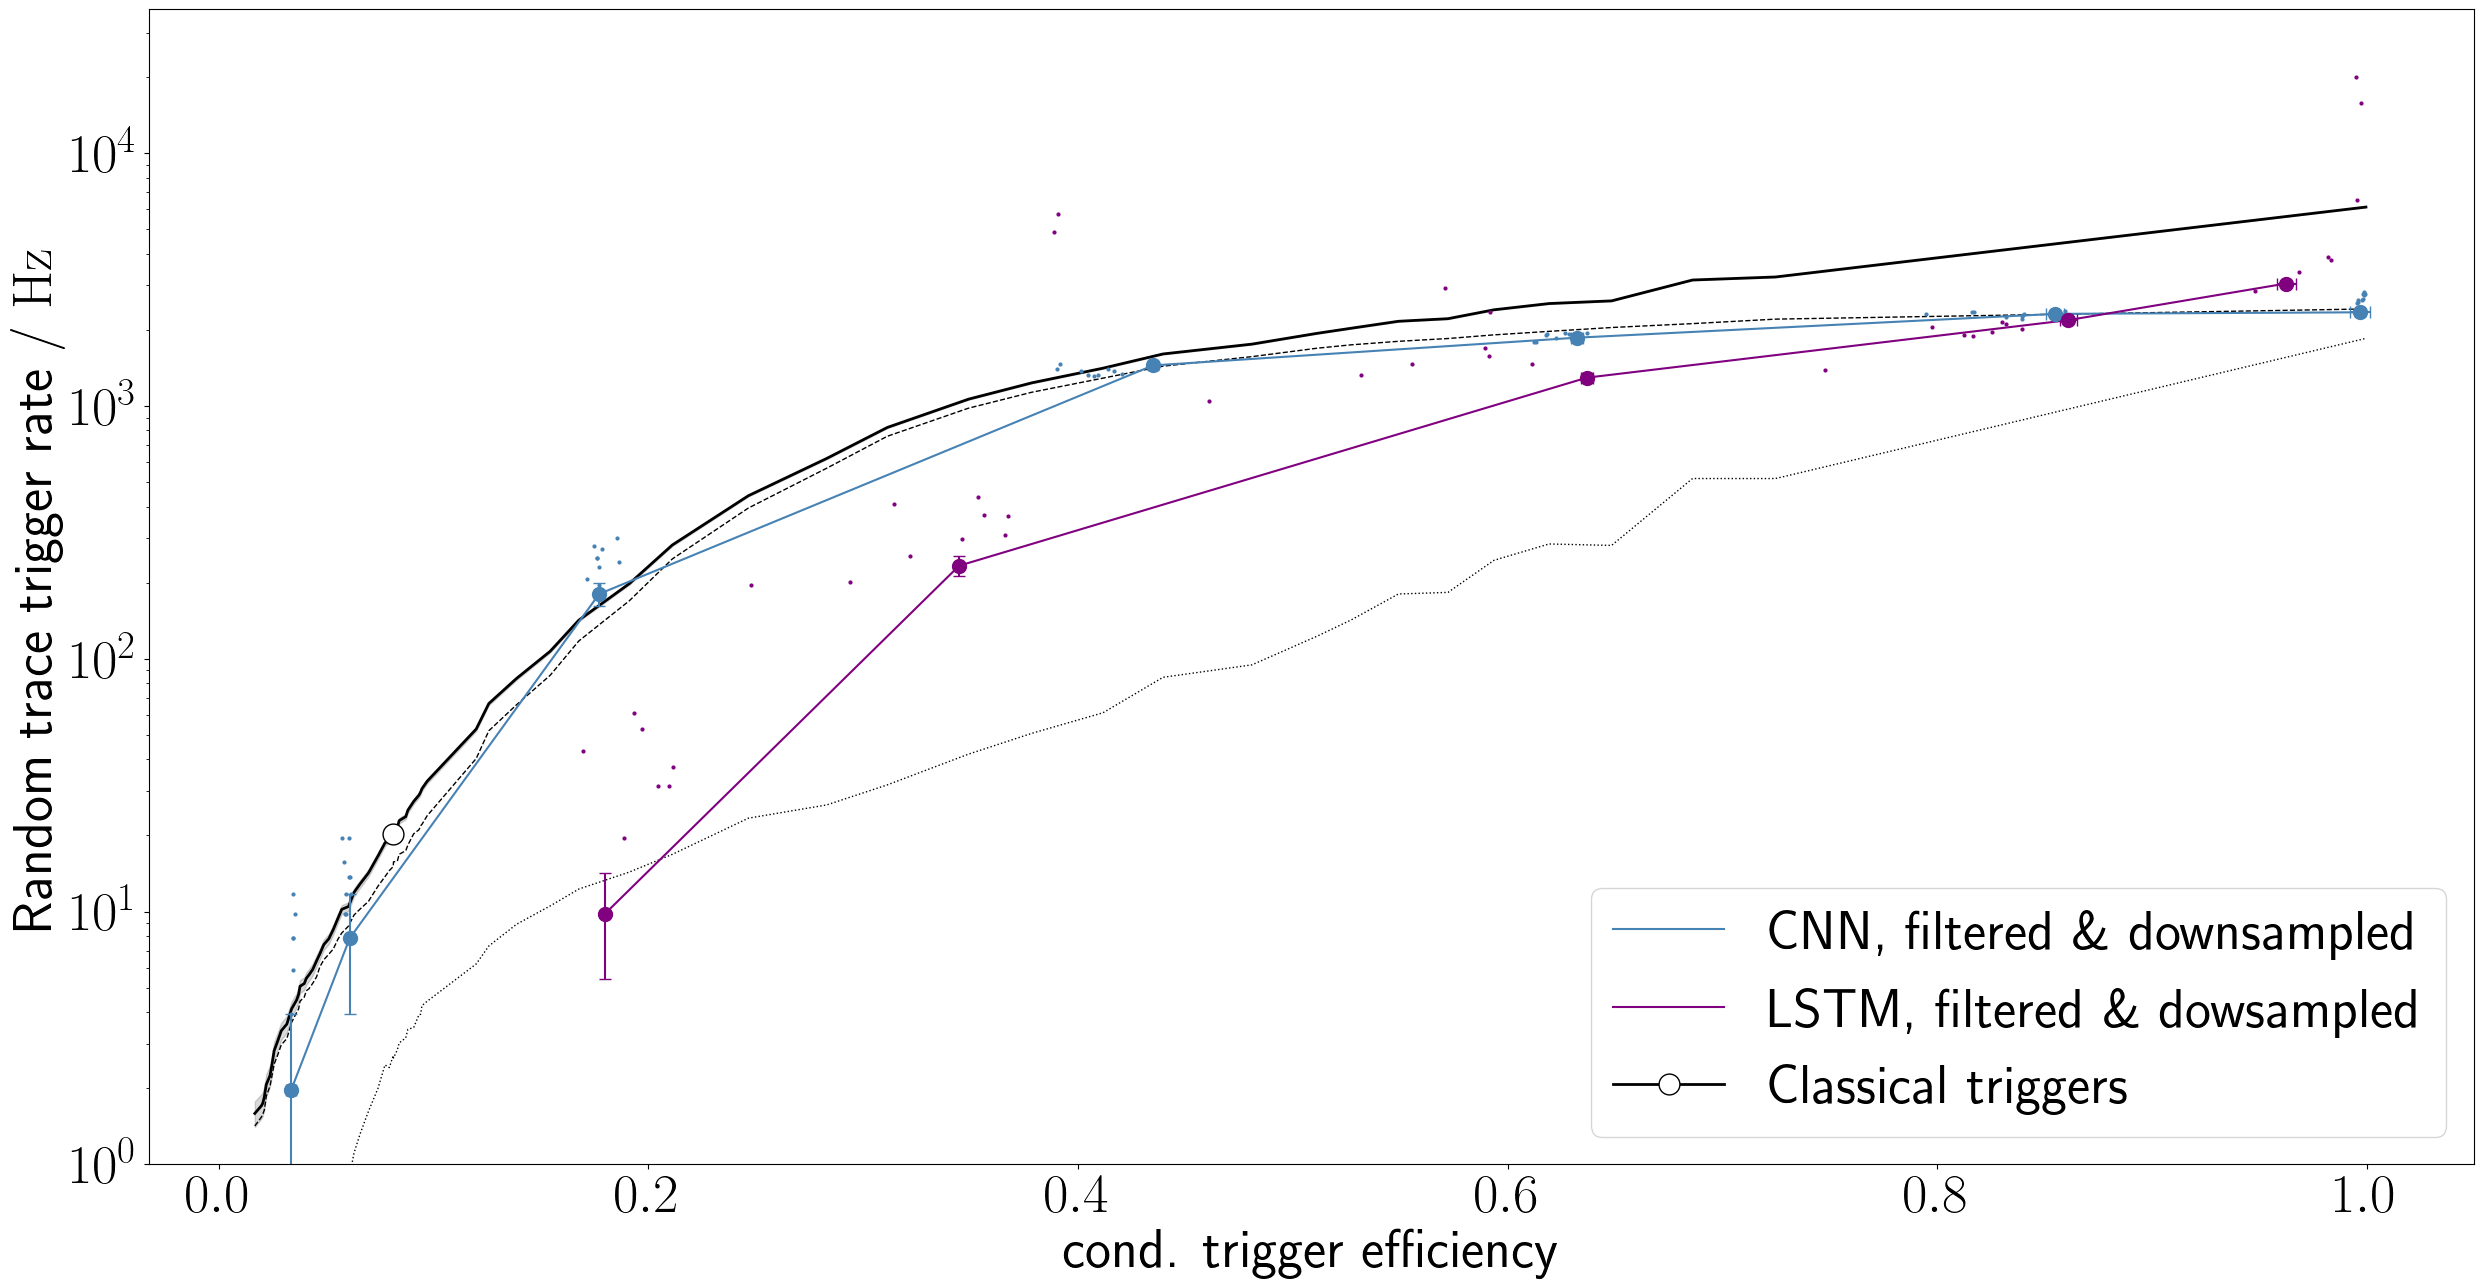
\includegraphics[width=0.9\textwidth]{./plots/LSTM_money_plot.png}
	\caption{LSTMs are consistently better than CNNs at charge thresholds $t_S > \SI{0.05}{\Charge}$. The purple line connects the best performing models (as 
	measured by network score $a$) for the ensembles with $t_S$ (from right to left) equal to $\SI{0.02}{\Charge}$, $\SI{0.05}{\Charge}$, $\SI{0.1}{\Charge}$,
	$\SI{0.2}{\Charge}$, and $\SI{0.5}{\Charge}$. At the highest examined cut $t_S = \SI{0.5}{\Charge}$, LSTMs show a score that is better than the ToT trigger.}
	\label{fig:LSTM-money-plot}
\end{figure}

\begin{figure}
	\centering
	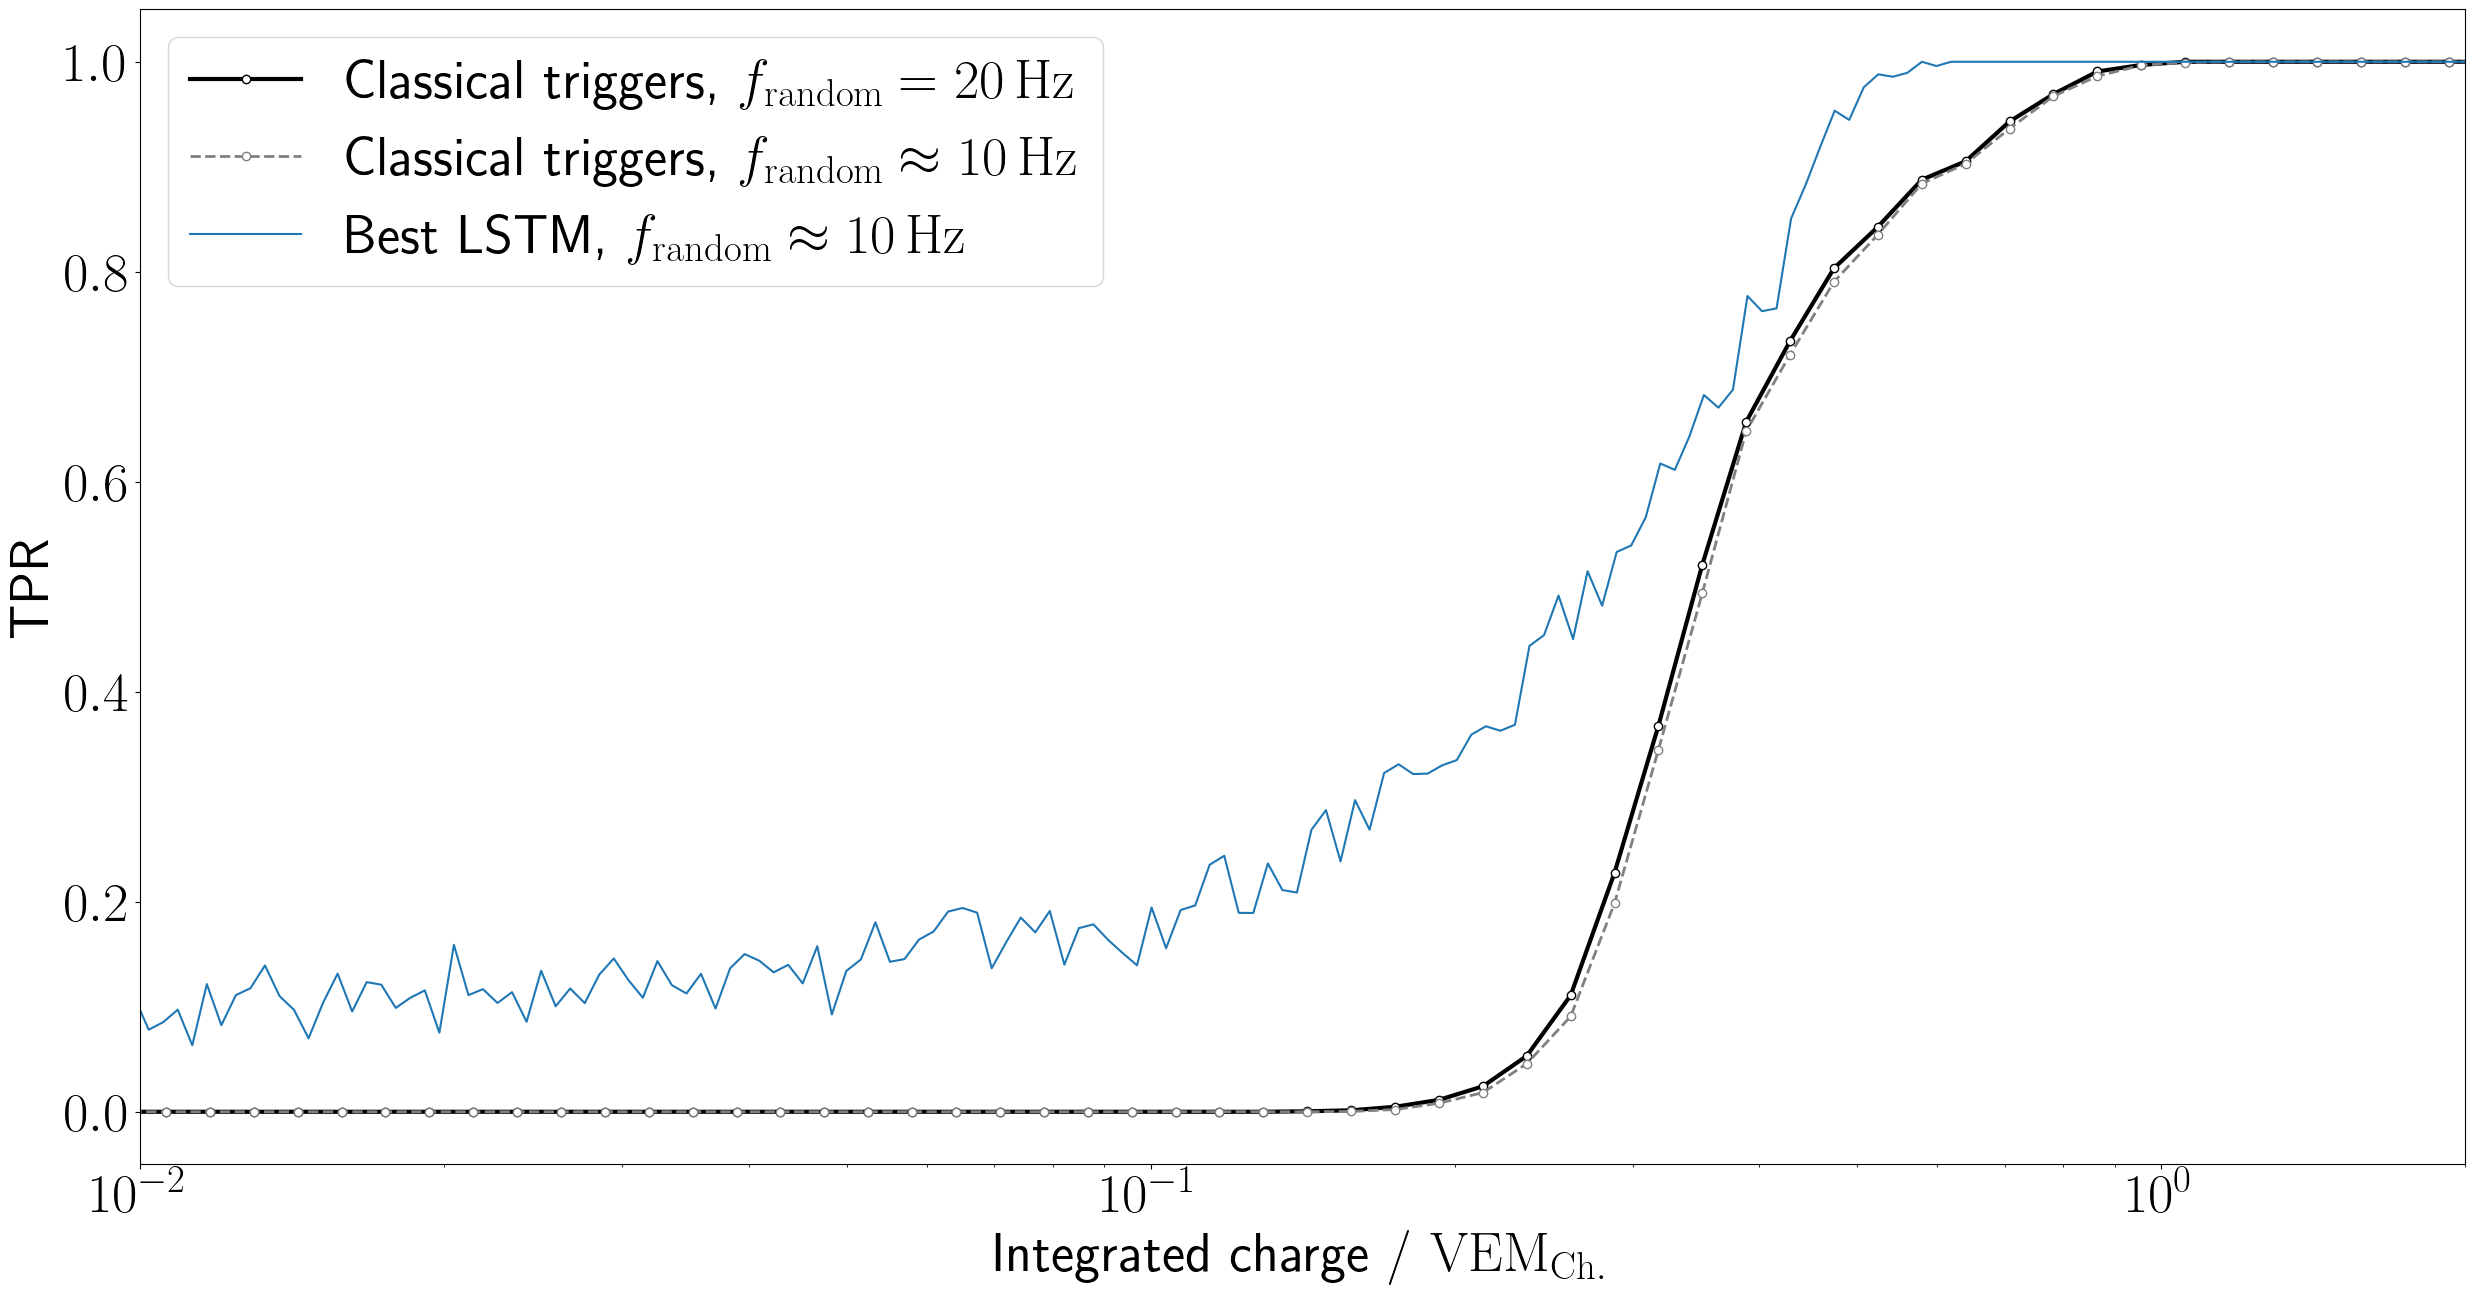
\includegraphics[width=0.9\textwidth]{./plots/LSTM_charge_TPR.png}
	\caption{The sensitivity of the best performing LSTM trained with $t_S = \SI{0.5}{\Charge}$ is superior to that of classical triggers for all deposited 
	signals. This is true both for the currently used classical trigger thresholds, for which $f_\text{random} = \SI{20}{\hertz}$, as well as for the direct 
	comparison of classical triggers with thresholds that yield the same trigger rate $f\text{random} \approx \SI{10}{\hertz}$ as the considered LSTM. Full 
	sensitivity, where all signals raise a T2 is reached at approximately $\SI{0.5}{\Charge}$.}
	\label{fig:LSTM-charge-TPR}
\end{figure}

\begin{figure}
	\centering
	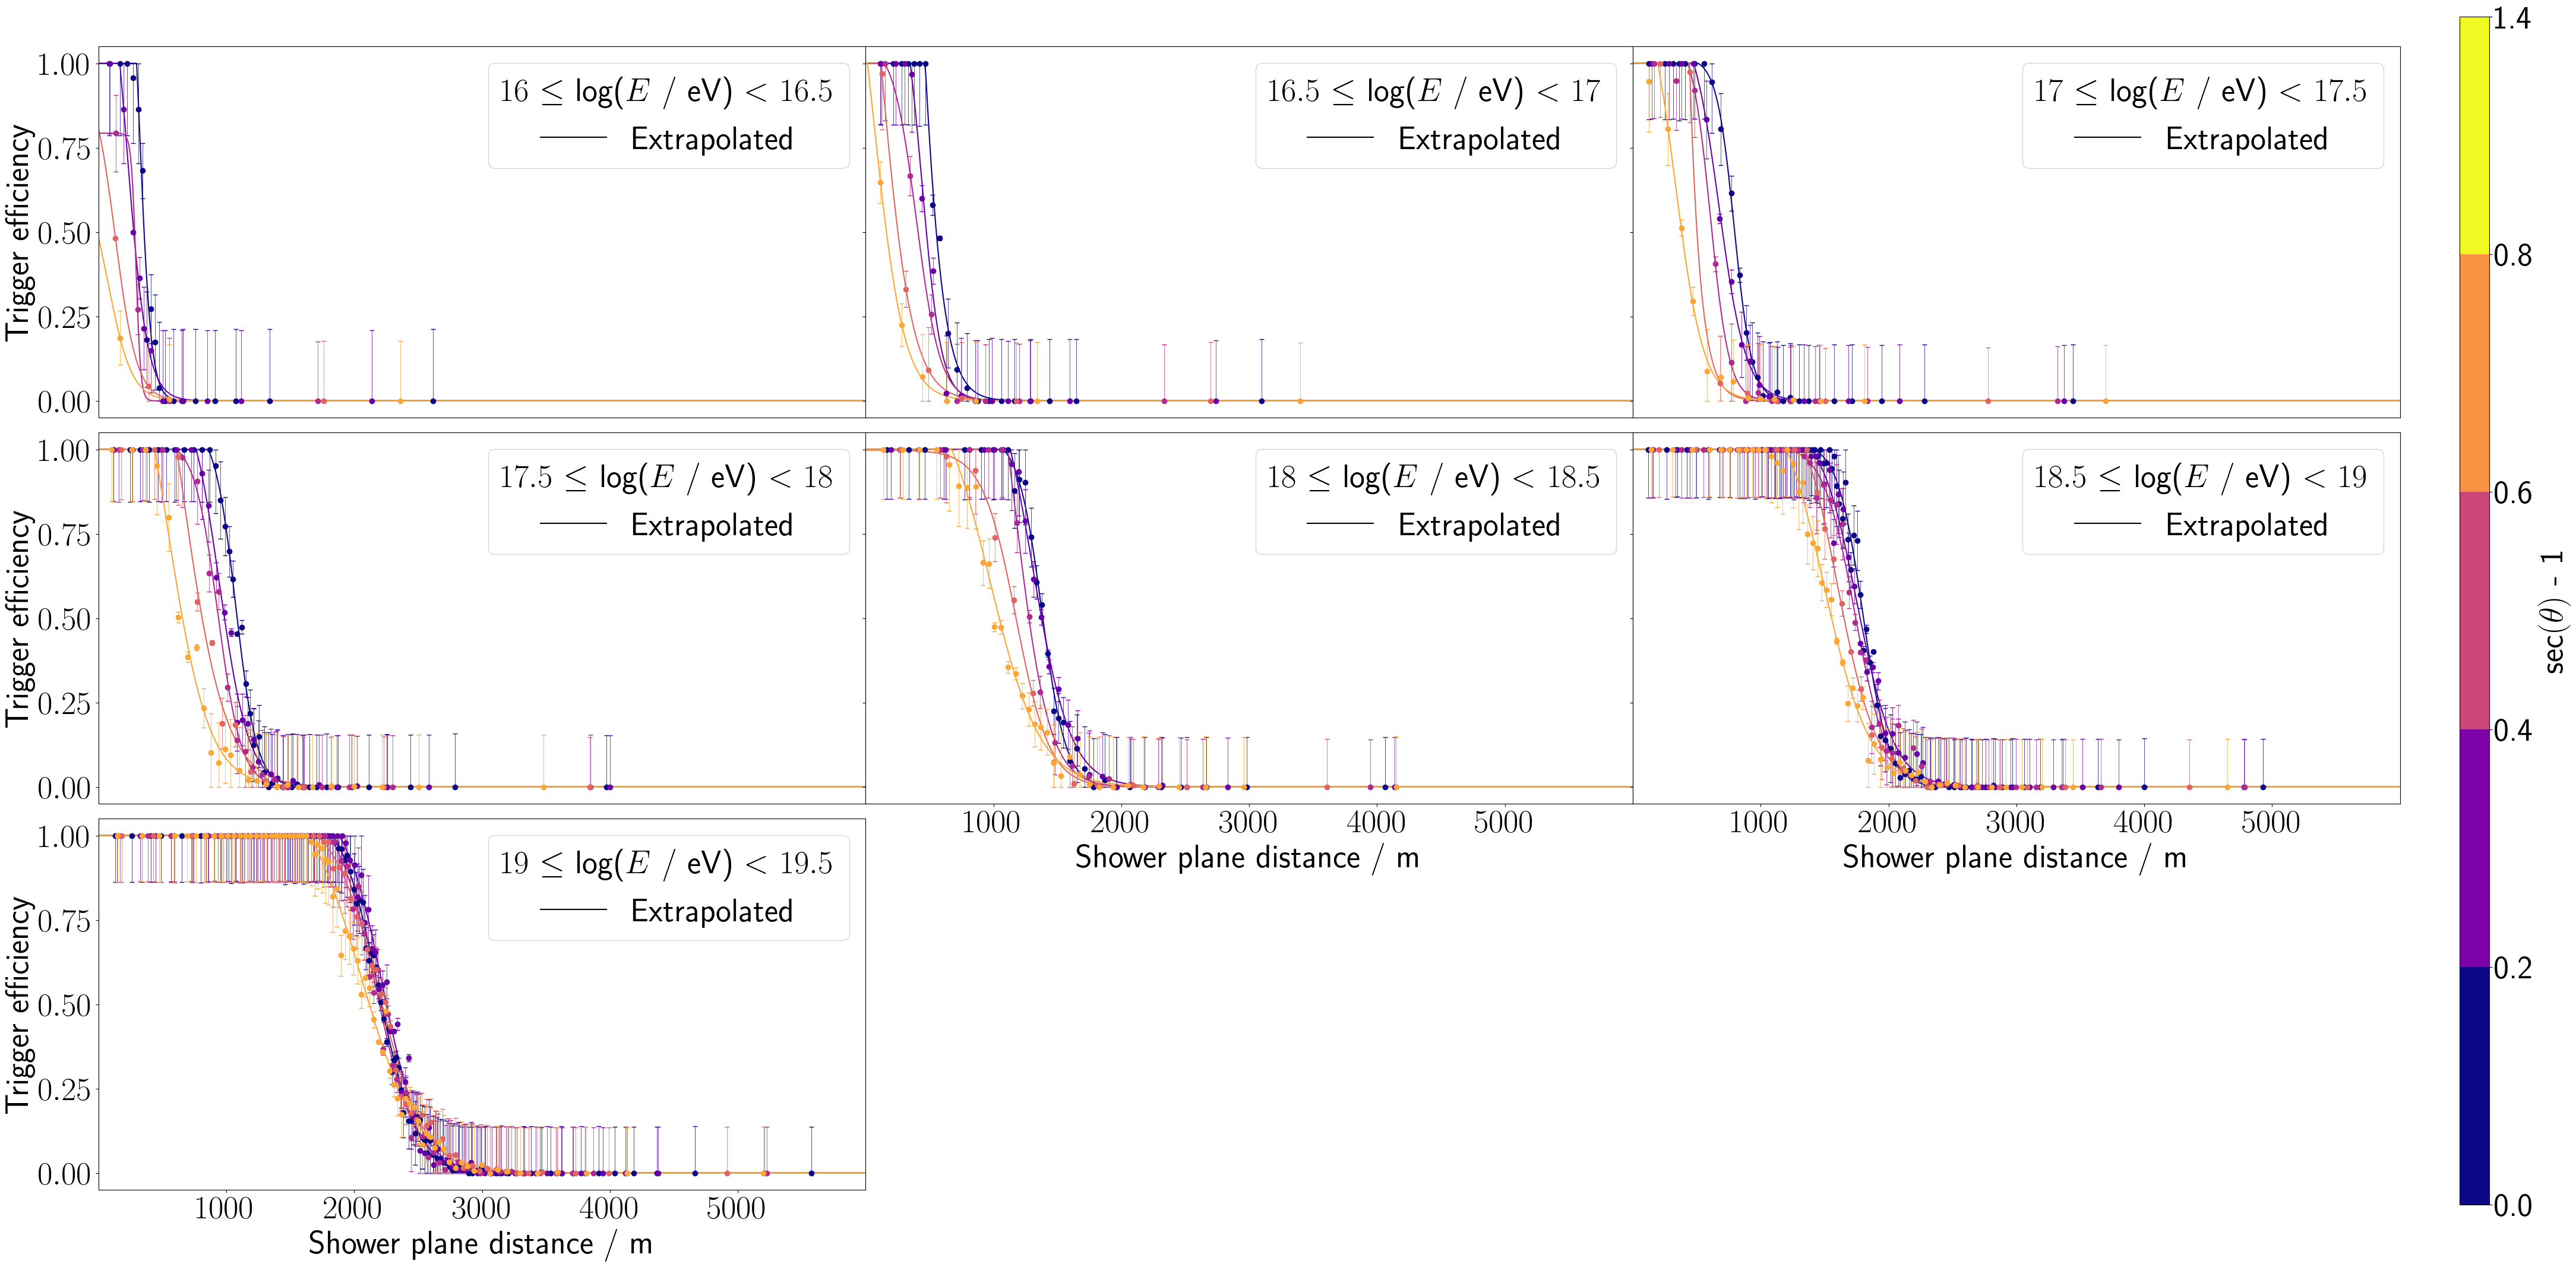
\includegraphics[width=0.9\textwidth]{./plots/LSTM_LTP.png}
	\caption{The lateral trigger probability for the best performing LSTM, where the classifier score $a$ as calculated in \autoref{eq:comparison-score} is 
	maximized. This is achieved by using a multi-layer LSTM trained with a charge cut $t_S = \SI{0.5}{\Charge}$.}
	\label{fig:LSTM-LTP}
\end{figure}

\begin{figure}
	\centering
	\includegraphics[width=0.9\textwidth]{./plots/LSTM_T3_efficiency.png}
	\caption{Resulting T3 efficiency of the best performing LSTM with charge cut $t_S = \SI{0.5}{\Charge}$, compared to classical T3 efficiency of the current 
	triggers operating with thresholds that yield the same random-trace trigger frequency. With a higher overall T3 efficiency, the LSTM trigger clearly shows a 
	higher signal to noise ratio.}
	\label{fig:LSTM-t3-efficiency}
\end{figure}

The potential of these multi-layer LSTMs seems promising. For classical triggers, a promise between acceptable background T2 rate and trigger efficiency must be 
found. The considered networks improve both aspects, and deliver a lower total T2 trigger rate while retaining a higher trigger efficiency. However, the necessity
of using three distinct layers over a single LSTM layer is not based on any reasoning. This issue may be indicative of the network architecture deciding
labels based on unphysical artifacts in the simulation data, and must be examined. By switching the ordering of the layers from $[1, 2, 3]$ to any possible 
permutation and recalculating labels for the validation dataset, possible shortcomings of the network should be revealed. The results of this analysis are shown 
in \autoref{fig:LSTM-permutations}, and find no clear trend or preferred ordering of layers. This implies that the LSTM architecture does in fact trigger on the 
physical information given as input, and not any artifact present in the data.

\begin{figure}
	\centering
	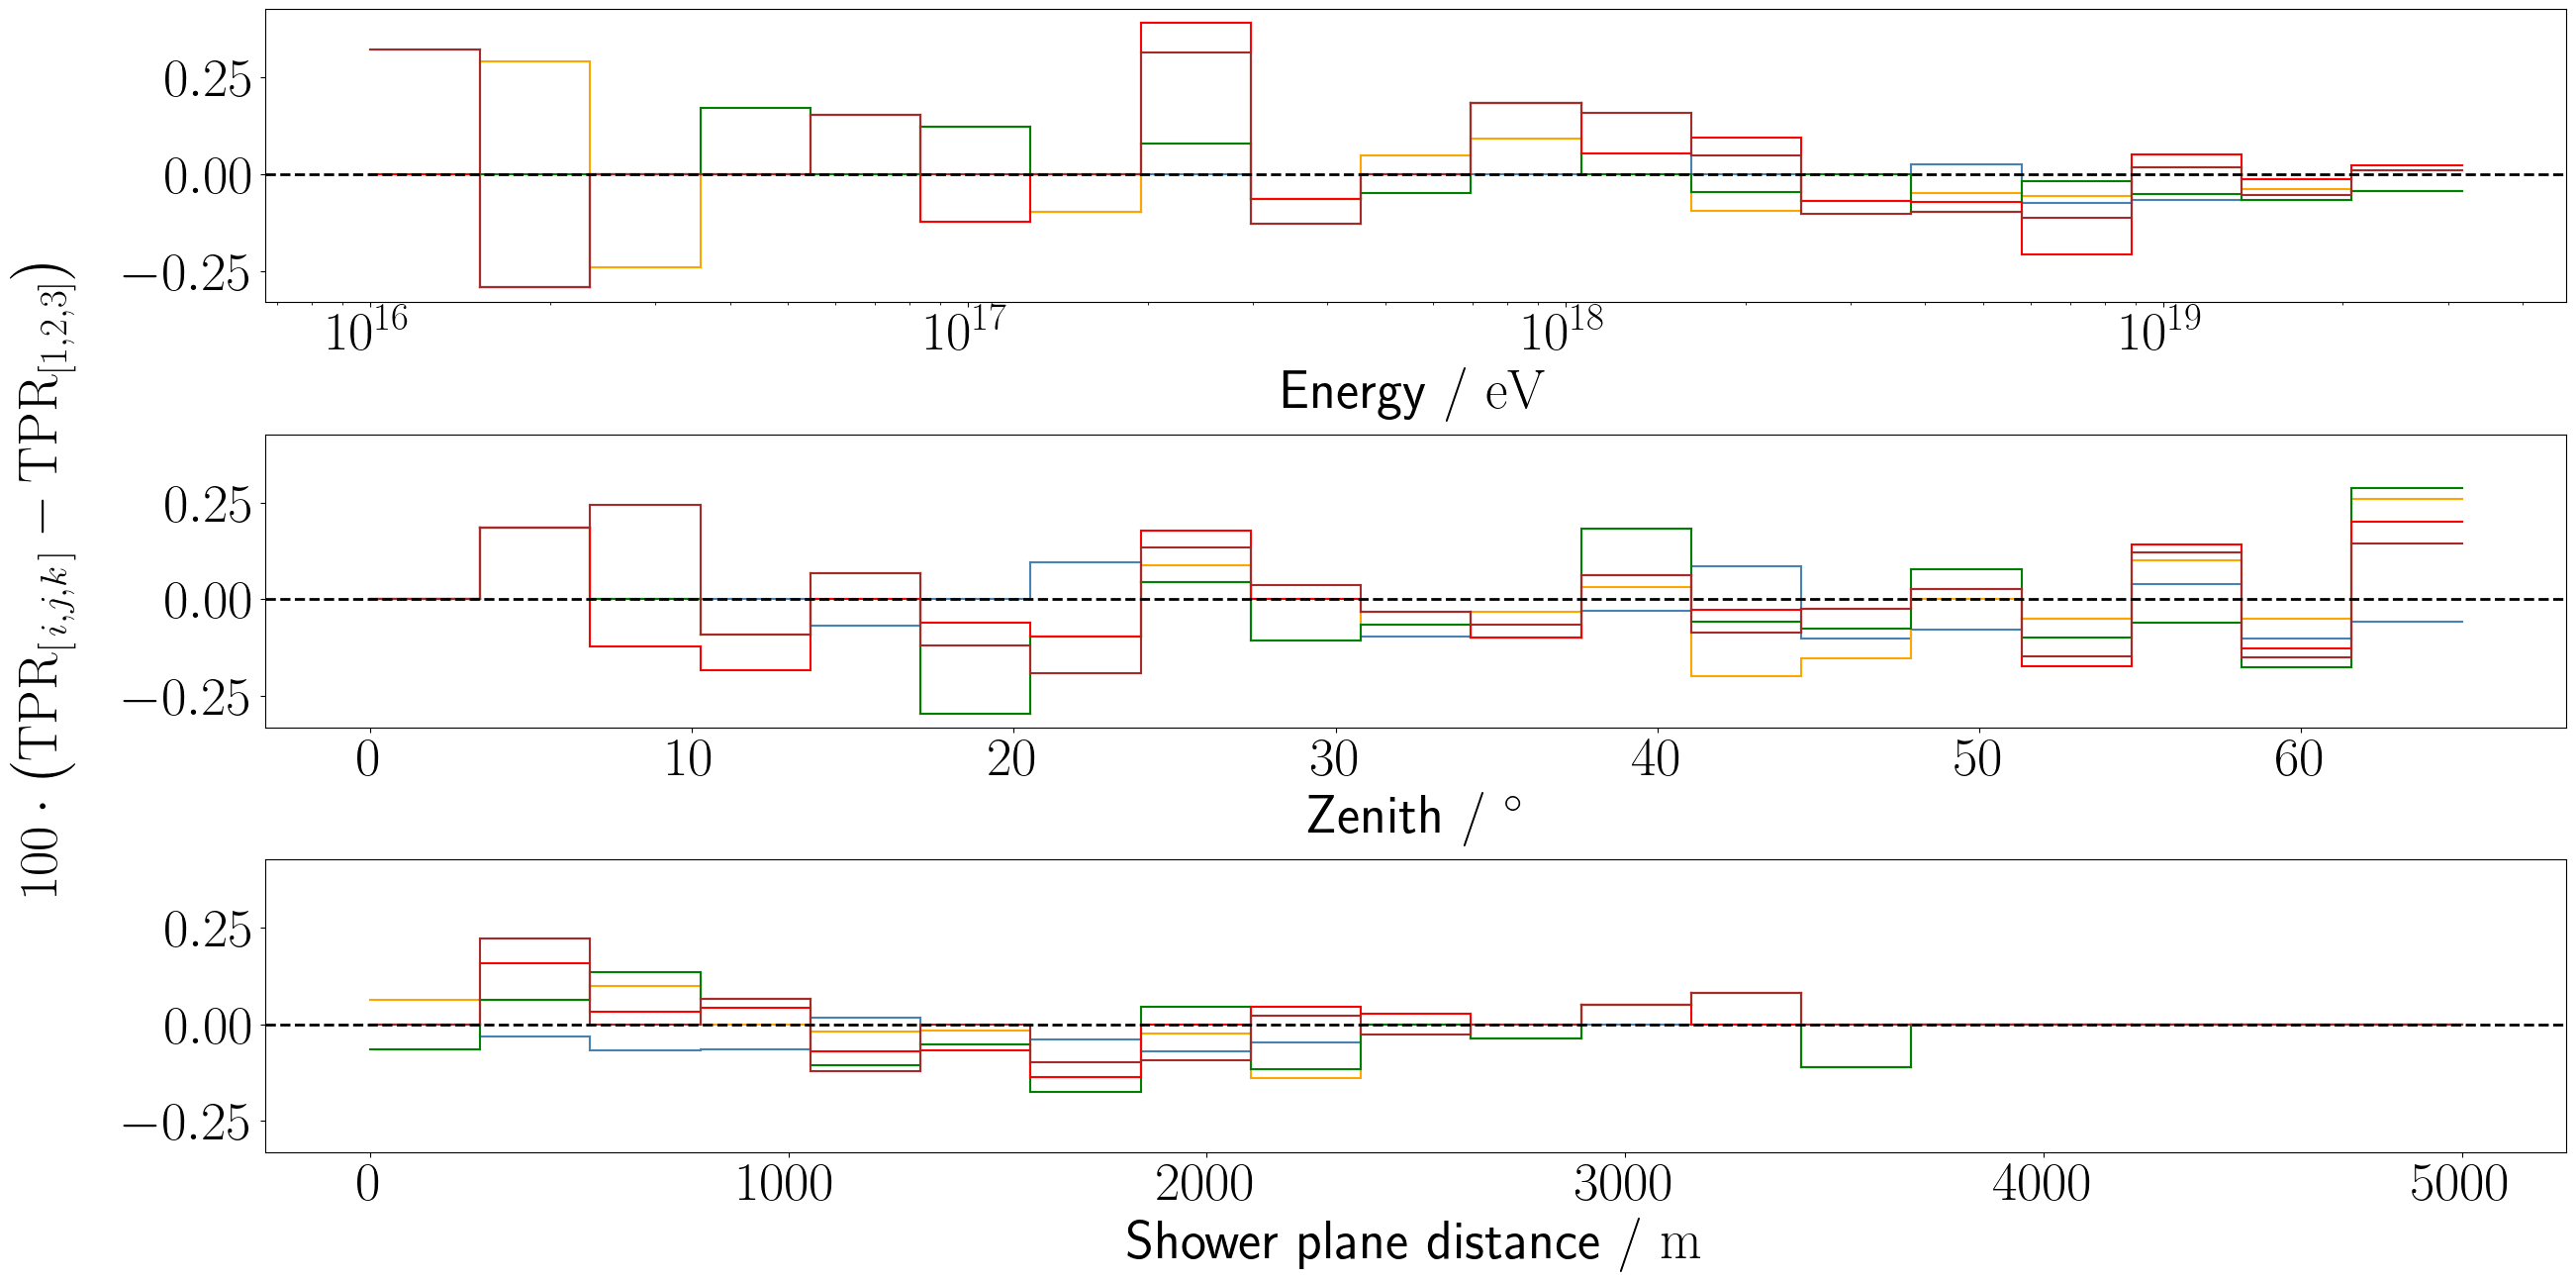
\includegraphics[width=0.9\textwidth]{./plots/LSTM_permutations.png}
	\caption{Absolute deviation of true positive rate between original layer ordering ($[1, 2, 3]$) and the five possible permutated architectures ($[1, 3, 2]$, 
	$[3, 1, 2]$, ...). No clear improvement/regression of performance is noted with respect to any shower variable. Peak deviations are on a sub-percent level.}
	\label{fig:LSTM-permutations}
\end{figure}